% Diplomový projekt 2017/2019
% Matúš Cuper

%-------------------------------------------------------------------------------
%   PACKAGES AND DOCUMENT CONFIGURATION
%-------------------------------------------------------------------------------

\documentclass[a4paper,twoside,slovak,12pt,appendix]{article}

\usepackage[slovak]{babel}                                                      % title in Slovak
\usepackage[IL2]{fontenc}                                                       % support for word wrapping of special Slovak characters at the end of line on the end
\usepackage[utf8]{inputenc}                                                     % support for special Slovak characters
\usepackage{enumitem}																														% support for itemize
\usepackage{times}																															% Times New Roman
\usepackage[hyphens]{url}                                                       % url in references
\usepackage[unicode]{hyperref}																									% hyperreferences in table of content
\usepackage{amsmath}                                                            % math fractions
\usepackage{amssymb}                                                            % real numbers sign
\usepackage{algorithm, algpseudocode}                                           % pseudocode writting
\usepackage{graphicx}                                                           % figures
\usepackage{multirow}																														% table with multirows
\usepackage{threeparttable}                                                     % table with footnotes
\usepackage{listings}                                                           % source code syntax highlighting
\usepackage{courier}																														% monospace in listings
\usepackage{caption}																														% enable caption centering
\usepackage{regexpatch}																													% fix slovak in table with multirows
\usepackage[titletoc]{appendix} 																								% appendix in toc with word appendix
\usepackage{dirtree}                                                            % directory tree in appendix
\usepackage[a4paper, centering,
											left=35mm, top=25mm, right=20mm, bottom=25mm]{geometry}		% set page margins

\makeatletter
\xpatchparametertext\@cline{-}{\cA-}{}{}																				% in slovak babel - is active character, it is necessary to escape it
\makeatother

\lstset{
    basicstyle=\ttfamily,
		breaklines=true,
    postbreak=\raisebox{0ex}[0ex][0ex]{\ensuremath{\color{red}\hookrightarrow\space}}
}

\graphicspath{ {img/} }		                                                      % set path for figures

\hypersetup{																																		% with default colours for links
    colorlinks,
		pageanchor=false,
    citecolor=black,
    filecolor=black,
    linkcolor=black,
    urlcolor=black
}

%-------------------------------------------------------------------------------
%   TITLE PAGES
%-------------------------------------------------------------------------------

\begin{document}
\begin{titlepage}
	\centering
	{\Large Slovenská technická univerzita v Bratislave \par}
	{\Large Fakulta informatiky a informačných technológií \par}
  \vspace{0.5cm}
  {\normalsize Evidenčné číslo: FIIT-182905-73688 \par}
	\vspace{7cm}
  {\large Bc. Matúš Cuper \par}
  \vspace{0.5cm}
	{\LARGE Identifikácia neštandardného správania odberateľov v~energetickej sieti \par}
	\vspace{0.5cm}
	{\large Diplomová práca \par}
	\vspace{7cm}
  \flushleft
	{\large Vedúci práce: Ing. Marek Lóderer \par}
  \vspace{0.5cm}
  {\large máj 2019 \par}
	\vfill
\end{titlepage}
\newpage\null\thispagestyle{empty}\newpage

\begin{titlepage}
	\centering
  {\Large Slovenská technická univerzita v Bratislave \par}
	{\Large Fakulta informatiky a informačných technológií \par}
  \vspace{0.5cm}
  {\normalsize Evidenčné číslo: FIIT-182905-73688 \par}
	\vspace{7cm}
  {\large Bc. Matúš Cuper \par}
  \vspace{0.5cm}
	{\LARGE Identifikácia neštandardného správania odberateľov v~energetickej sieti \par}
	\vspace{0.5cm}
	{\large Diplomová práca \\}
	\vspace{7cm}
  \flushleft
  {\normalsize Študijný program: Inteligentné softvérové systémy \par}
	{\normalsize Študijný odbor: 9.2.5 Softvérové inžinierstvo, 9.2.8 Umelá inteligencia \par}
	{\normalsize Miesto vypracovania: Ústav informatiky a softvérového inžinierstva, FIIT STU v Bratislave \par}
	{\normalsize Vedúci práce: Ing. Marek Lóderer \par}
  \vspace{0.5cm}
  {\normalsize máj 2019 \par}
\end{titlepage}
\newpage\null\thispagestyle{empty}\newpage

%-------------------------------------------------------------------------------
%   ANOTATION
%-------------------------------------------------------------------------------

% \newpage\null\thispagestyle{empty}\newpage

\begin{titlepage}
\begin{center}
  {\small Slovenská technická univerzita v Bratislave \par}
  {\small \textbf{FAKULTA INFORMATIKY A INFORMAČNÝCH TECHNOLÓGIÍ}}
  \rule{\textwidth}{1pt}

  \vspace*{1.5cm}
  \begin{Large}
    \textbf{Anotácia} \par
  \end{Large}
\end{center}
{Slovenská technická univerzita v Bratislave \par}
{FAKULTA INFORMATIKY A INFORMAČNÝCH TECHNOLÓGIÍ \par}
{Študijný program: Inteligentné softvérové systémy \par}
{Autor: Bc. Matúš Cuper \par}
{Bakalárska práca: Identifikácia neštandardného správania odberateľov v~energetickej sieti \par}
{Vedúci práce: Ing. Marek Lóderer \par}
{máj 2019 \par}
\bigskip
V práci sme sa zamerali na identifikáciu anomálií v~energetických časových
radoch. Anomálie môžu vznikať na základe neštandardného správania odberateľov
alebo poruchy inteligentného merača spotreby elektrickej energie. Cieľom
diplomovej práce je identifikovať oba takéto prípady a~znížiť tak straty
distribučnej spoločnosti. Zároveň je nutné identifikovať iba také prípady, kedy
sa jedná o~dočasnú zmenu v~správaní, či už je to dôsledkom zmeny počtu
obyvateľov, počasia alebo výnimočnou udalosťou. So vznikajúcimi technológiami
sa postupne mení aj profil spotreby odberateľov, a~preto je nutné správne
identifikovať aj nové trendy v~dátach.

Analyzovali sme časové rady, anomálie a~používané metódy na ich identifikáciu.
Opísali sme problémy, ktoré vznikajú pri identifikácií anomálií v~doméne
energetiky, a~ktorým musí čeliť aj naša metóda. Bližšie sme sa zamerali na
zhlukovanie časových radov, ktoré prináša nové prístupy do zhlukovania
vysokodimenzionálnych dát, medzi ktoré patrí aj vyhladzovanie, redukcia dimenzií
alebo selekcia atribútov. Navrhovaná metóda zlúči diskretizované vyhladené
časové rady a~následne sú identifikované anomálie na základe vytvorených zhlukov
a~rozloženia profilu používateľa v~zhlukoch.
\end{titlepage}
\newpage\null\thispagestyle{empty}\newpage

\begin{titlepage}
\begin{center}
  {\small Slovak University of Technology Bratislava \par}
  {\small \textbf{FACULTY OF INFORMATICS AND INFORMATION TECHNOLOGIES}}
  \rule{\textwidth}{1pt}

  \vspace*{1.5cm}
  \begin{Large}
    \textbf{Annotation} \par
  \end{Large}
\end{center}
{Slovak University of Technology Bratislava \par}
{FACULTY OF INFORMATICS AND INFORMATION TECHNOLOGIES \par}
{Degree Course: Intelligent software systems \par}
{Author: Bc. Matúš Cuper \par}
{Bachelor thesis: Identification of abnormal behavior of customers in the power grid \par}
{Supervisor: Ing. Marek Lóderer \par}
{May 2019 \par}
\bigskip
In the thesis we focused on anomaly identification in energy time series.
Anomalies can be caused by abnormal behavior of customers or failure of
intelligent meter of electricity load. The aim of this master thesis is to
identify these mentioned cases and reduce electricity loss of distribution
company. Also it is necessary to identify only cases, when the behavioral change
is temporal, whether it is result of different number of residents, weather or
an exceptional occasion. Nowadays, electricity load profile of customers is
changing as the new technologies are involved and therefore it is necessary to
correctly identify new trends in data.

We also analyzed time series, anomalies and methods used for their
identification. We described problems linked to identifications of anomalies in
domain of electricity, while our method is facing these problems as well. We
focused on time series clustering, which brings new approaches to clustering of
multidimensional data, which includes also smoothing, dimension reduction and
attribute selection. Proposed method clusters discretized smoothed time series
and then, based on created clusters and layout of customers profile in cluster,
identifies anomalies.
\end{titlepage}
\newpage\null\thispagestyle{empty}\newpage

%-------------------------------------------------------------------------------
%   Declaration
%-------------------------------------------------------------------------------

\begin{titlepage}
\vspace*{15cm}
\begin{large}
  \noindent \textbf{ČESTNÉ PREHLÁSENIE} \par
\end{large}
\vspace*{0.5cm}
\noindent
Čestne prehlasujem, že diplomovú prácu som vypracoval samostatne pod vedením
vedúceho diplomovej práce a s použitím odbornej literatúry, ktorá je uvedená
v zozname použitej literatúry. \\
\vspace*{0.5cm}\\
\hspace*{10cm}............................\\
\hspace*{10.7cm} Matúš Cuper
\end{titlepage}
\newpage\null\thispagestyle{empty}\newpage

\begin{titlepage}
\vspace*{15cm}
\begin{large}
  \noindent \textbf{POĎAKOVANIE} \par
\end{large}
\vspace*{0.5cm}
\noindent
Ďakujem vedúcemu diplomovej práce Ing. Marekovi Lódererovi za odborné vedenie,
cenné rady a pripomienky pri spracovaní diplomovej práce.
\end{titlepage}
\newpage\null\thispagestyle{empty}\newpage

%-------------------------------------------------------------------------------
%   Table of contents
%-------------------------------------------------------------------------------

\newpage
\tableofcontents
\thispagestyle{empty}                                                           % removes page numbering from table of contents page

% \newpage
% \listoffigures
% \thispagestyle{empty}
%
% \newpage
% \listoftables
% \thispagestyle{empty}

%-------------------------------------------------------------------------------
%   Chapter 1 - Introduction
%-------------------------------------------------------------------------------

% \newpage\null\thispagestyle{empty}
\newpage
\setcounter{page}{1}
\section{Úvod}
Jedným z~problémov, ktorým v~súčasnosti čelia distribučné spoločnosti, je
detekcia neštandardného správania odberateľov. Jej úlohou je identifikovať
profily zákazníkov, ktorí svojím správaním porušujú stanovené podmienky
a~manipulujú s~hodnotami nameranými meračmi za cieľom obohatenia sa. Samozrejme
tiež dochádza k~prípadom, kedy je presnosť meracieho zariadenia nižšia aj bez
zapríčinenia zákazníka. Oba prípady sú pre distribučnú spoločnosť nežiaduce a~je
v~záujme zníženia strát, ich čo najskôr identifikovať. Obvykle sú za týmto
účelom vykonávané náhodné kontroly, ktoré pokrývajú iba nízky počet zákazníkov
s~anomálnym správaním. Na základe množstva dát získavaných z~inteligentných
meračov je možné modelovať správanie zákazníkov. Distribučné spoločnosti tak
môžu znižovať svoje straty a~preverovať iba odberateľov, ktorí svojím profilom
nezapadajú medzi odberateľov so štandardným správaním.

% TODO dopíš niečo o anomáliách a predpovediach časových radov
% TODO výsledky práce
% TODO členenie práce
\newpage\null\thispagestyle{empty}\newpage

%-------------------------------------------------------------------------------
%   Chapter 2 - Problem analysis
%-------------------------------------------------------------------------------

\newpage
\section{Analýza problému}
\label{c:problem-analysis}
Tak ako je spomenuté v~článku~\cite{Meffe2009}, straty v~distribučných sieťach
v~niektorých krajinách tvoria až 30\% z~celkového objemu distribuovanej energie.
Väčšinu strát vytvára svojimi vlastnosťami samotná sieť, no nezanedbateľnú časť
tvoria aj nelegálne odbery. Pravidelná kontrola všetkých odberateľov by bola
časovo aj finančne náročná, preto je potrebné správne identifikovať zákazníkov
s~neštandardnou spotrebou energie, čím sa minimalizujú náklady spojené
s~kontrolami. Zatiaľ čo v~minulosti bola možná identifikácia nelegálnych odberov
len fyzickou kontrolou, dnes vieme obmedziť okruh podozrivých aj na diaľku,
keďže inteligentné merače nám poskytujú dáta v~pravidelných intervaloch
s~minimálnou odchýlkou.

Vďaka tomu vznikajú nové možnosti identifikácie neštandardného správania
využitím dátovej analytiky a~strojového učenia. Zatiaľ čo väčšina algoritmov na
identifikáciu anomálií pracuje s~nízkorozmernými dátami, časové rady predstavujú
presný opak a~použité metódy sa líšia od tých klasických. Výzvou pri skupinových
a~kontextových anomáliách je aj vhodný výber premenných, na základe ktorých budú
anomálie identifikované. Zvýšenie presnosti pri hľadaní anomálií môžeme docieliť
kombinovaním rôznych zdrojov dát, či už by sa jednalo o~počasie alebo údaje
z~inteligentných meračov iných druhov energie. Cieľom tejto kapitoly je preto
analyzovať a~porovnať používané metódy pri detekcii anomálií v~časových radoch
a~zamerať sa najmä na vhodnú reprezentáciu jednotlivých odberateľov pomocou
získaných dát.

%-------------------------------------------------------------------------------
%   Time series
%-------------------------------------------------------------------------------

\subsection{Časové rady}
Merania časových radov predstavujú množinu dátových bodov, usporiadané
v~chronologickom poradí. Takúto množinu môžeme definovať ako množinu vektorov
$x(t)$, kde premenná $x$ predstavuje časový rad a~$t$ čas, kedy bolo meranie
vykonané. Časové rady pozostávajúce z~meraní jednej veličiny sa nazývajú
jednorozmerné, pri meraní viacerých veličín sa jedná o~viacrozmerné časové rady.
Tiež ich môžeme rozdeliť na spojité a~diskrétne. Spojité časové rady merajú
pozorovanú veličinu v~každej jednotke času. Môže sa jednať napr. o~počasie,
veľkosť prietoku rieky alebo koncentráciu látok pri chemických procesoch.
Diskrétne časové rady sú pozorované spravidla v~rovnakých časových intervaloch,
napr. rokoch, dňoch či minútach. Stretnúť sa s~nimi môžeme pri kurzoch mien,
produkcii štátov či spotrebe elektrickej energie~\cite{Agrawal2013}.

%-------------------------------------------------------------------------------
%   Time series analysis
%-------------------------------------------------------------------------------

\subsubsection{Analýza časových radov}
Časové rady môžeme reprezentovať pomocou matematického modelu, ktorého parametre
sú dané nameranými dátami. Parametre sú určené na základe dátovej analýzy
nazhromaždených dát. Cieľom je určiť parametre tak, aby predikcia výsledného
modelu bola čo najpresnejšia. Proces analýzy a~úpravy parametrov je možné
opakovať pokiaľ model nedosahuje dostatočne uspokojivé
výsledky~\cite{Agrawal2013}.

Premenná $\hat{x}$ vo vzorci~\ref{eq:time-series} predstavuje predikovanú
hodnotu časového radu $x$. Cieľom je nájsť funkciu $f(x)$, ktorá predikuje
budúce hodnoty časového radu $x$ tak, aby boli čo najpresnejšie, konzistentné
a~objektívne~\cite{Sapankevych2009}.

\begin{equation}
  \hat{x}(t+\Delta_t) = f(x(t-a), x(t-b), x(t-c), ...)
  \label{eq:time-series}
\end{equation}

%-------------------------------------------------------------------------------
%   Time series components
%-------------------------------------------------------------------------------

\subsubsection{Zložky časových radov}
Na vývoj časových radov vplývajú ich jednotlivé komponenty, z~ktorých
pozostávajú. Ich vývoj je ovplyvnení rôznymi faktormi, či už ekonomickými,
ekologickými, počasím, sviatkami alebo kultúrou. Priebehy grafov jednotlivých
komponentov potom môžu byť cyklické, rastúce, klesajúce alebo stagnujúce
v~závislosti od toho, či existuje zmena, ktorá je trvalá alebo opakujúca.
Taktiež aj veľkosť periódy tohto cyklu môže byť rôzna, a~to niekoľko dní,
mesiacov či rokov. Keďže prostredie, v~ktorom meriame predpovedanú veličinu sa
vyvíja, rovnako sa vyvíja aj správanie pozorovanej veličiny. Preto je potrebné
pri modelovaní správania uvažovať jednotlivé komponenty časového radu.
V~literatúre sa najčastejšie stretávame s~rozdelením na 4~komponenty, a~to
trendovú, cyklickú, sezónnu a~reziduálnu zložku~\cite{Grmanova2016}.

\paragraph{Trendová zložka} zastupuje dlhodobé správanie časového radu. Ide
o~dlhodobé klesanie, rast alebo stagnáciu časového radu. Príkladom môže byť
neustále predlžovanie priemernej doby dožitia alebo aj rast svetovej populácie.
Priebeh dekompovanej trendovej zložky môžeme vidieť na
obrázku~\ref{fig:trend-component}~\cite{Agrawal2013}.

\begin{figure}[H]
  \centering
  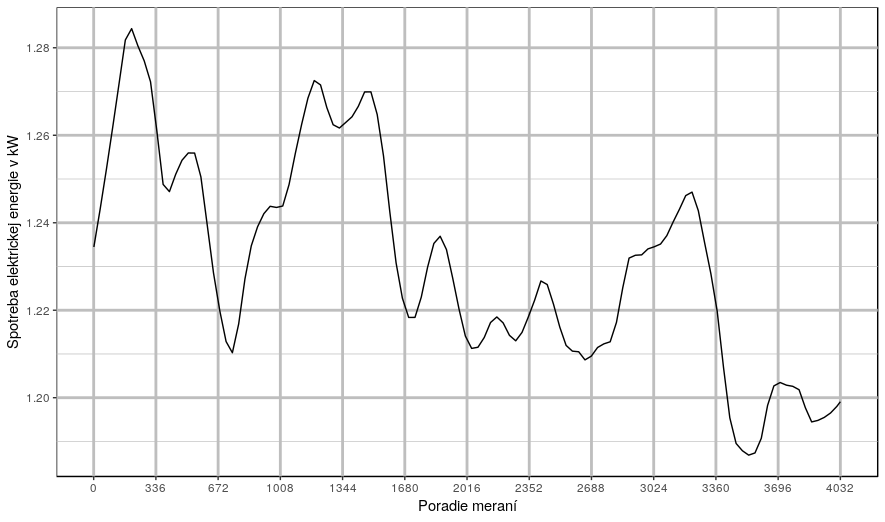
\includegraphics[width=\textwidth]{trend_component.png}
  \caption{Príklad trendovej zložky časového radu.}
  \label{fig:trend-component}
\end{figure}

\paragraph{Cyklická zložka} predstavuje strednodobú opakujúcu sa zmenu.
Najčastejšie sa pri tom jedná o~obdobie 2~a~viac rokov. Táto zložka býva výrazne
zastúpená pri ekonomických a~finančných časových radoch. Príkladom môže byť
aj podnikateľský cyklus, ktorý pozostáva zo 4~opakujúcich sa
fáz~\cite{Agrawal2013}.

\paragraph{Sezónna zložka} sa počas roka mení a~predstavuje tak striedanie
ročných období. Priebeh funkcie je ovplyvňovaný najmä podnebnými podmienkami
a~počasím, ale aj kultúrou, náboženstvom či tradíciami. Príkladom môže byť
predaj sezónnych výrobkov, ktorý sa počas roka výrazne mení. Priebeh funkcie
dekomponovanej zložky môžeme vidieť na
obrázku~\ref{fig:seasonal-component}~\cite{Agrawal2013}.

\begin{figure}[H]
  \centering
  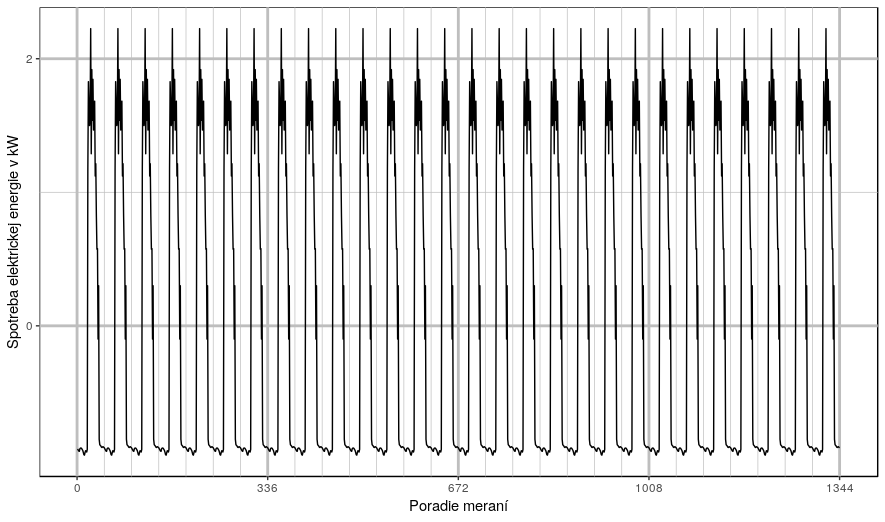
\includegraphics[width=\textwidth]{season_component.png}
  \caption{Príklad sezónnej zložky časového radu.}
  \label{fig:seasonal-component}
\end{figure}

\paragraph{Reziduálna zložka} v~literatúre často označovaná aj ako náhodná
zložka alebo biely šum, predstavuje nepredvídateľnú veličinu, ktorá
nesystematicky ovplyvňuje pozorovaný časový rad. Metóda jej merania zatiaľ nie
je v štatistike definovaná. Priebeh funkcie nemá žiadny vzor a~môže vznikať na
základe prírodných katastrof, ale aj nepredvídateľnej zhody náhod. Príklad
priebehu môže byť aj graf znázornený na
obrázku~\ref{fig:random-component}~\cite{Agrawal2013}.

\begin{figure}[H]
  \centering
  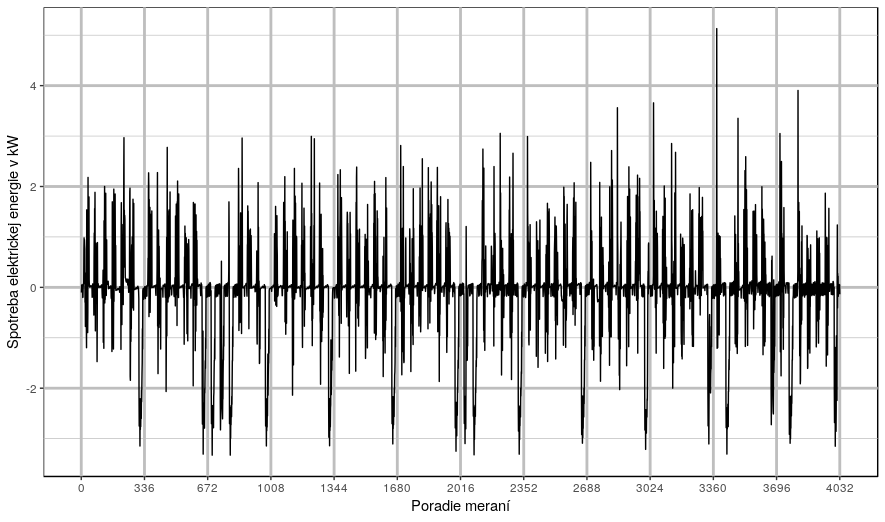
\includegraphics[width=\textwidth]{random_component.png}
  \caption{Príklad reziduálnej zložky časového radu.}
  \label{fig:random-component}
\end{figure}

\subsubsection{Typy modelov časových radov}
Kombináciou komponentov časových radov identifikovaných v~predchádzajúcej
kapitole vznikajú 2~typy modelov, aditívny a~multiplikatívny.

\begin{equation}
  \begin{split}
    Y(t) = T(t) \times S(t) \times C(t) \times I(t)
    \\
    Y(t) = T(t) + S(t) + C(t) + I(t)
  \end{split}
  \label{eq:time-series-models}
\end{equation}

Vo vzorci~\ref{eq:time-series-models}, $Y(t)$ predstavuje meranie pozorovanej
veličiny v~čase $t$. Ostatné premenné $T$, $S$, $C$ a $I$ reprezentujú trendový,
sezónny, cyklický a~reziduálny komponent. Veličiny multiplikatívneho modelu sa
môžu vzájomne ovplyvňovať, zatiaľ čo pri aditívnom modely predpokladáme ich
nezávislosť. Multiplikatívny model je znázornený na
obrázku~\ref{fig:multi-time-series-model} a~aditívny na
obrázku~\ref{fig:add-time-series-model}~\cite{Agrawal2013}.

\begin{figure}[H]
  \centering
	\captionsetup{justification=centering}
  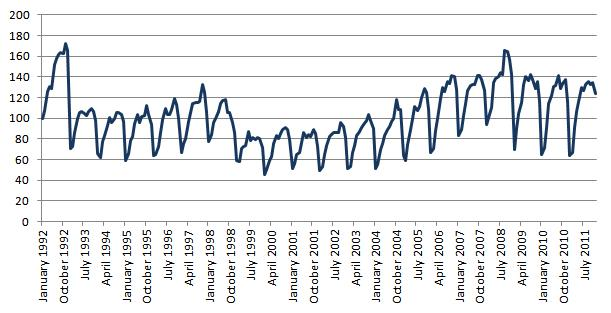
\includegraphics[width=\textwidth]{multi_model.jpg}
  \caption[Príklad multiplikatívneho modelu.]{Príklad multiplikatívneho modelu, index stavebnej produkcie Slovenska, Eurostat.}
  \label{fig:multi-time-series-model}
\end{figure}

\begin{figure}[H]
  \centering
  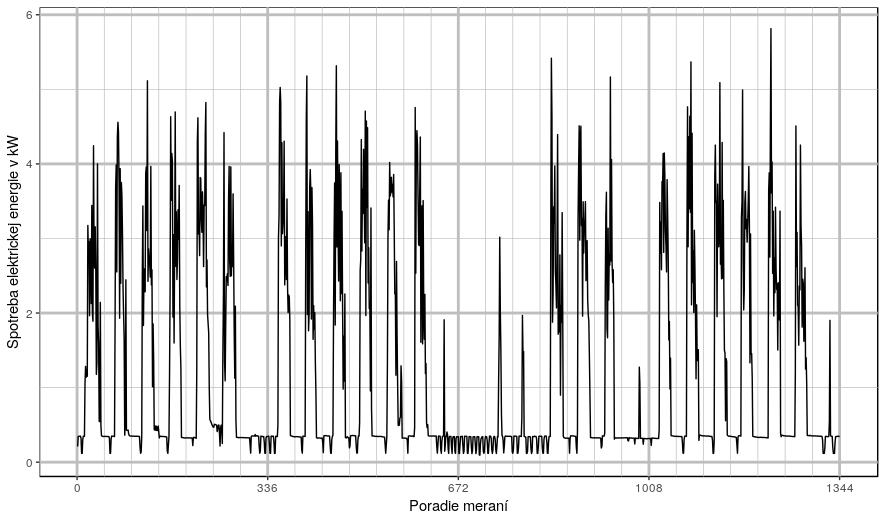
\includegraphics[width=0.9\textwidth]{add_model.png}
  \caption[Príklad aditívneho modelu.]{Príklad aditívneho modelu, spotreba elektrickej energie v~regióne, Slovensko.}
  \label{fig:add-time-series-model}
\end{figure}

%-------------------------------------------------------------------------------
%   Division of time series
%-------------------------------------------------------------------------------

\subsubsection{Delenie časových radov}
Výraznými vlastnosťami časových radov sú aj synchrónnosť a~periodicita,
znázornená na
obrázkoch~\ref{fig:periodic-time-series}~a~\ref{fig:non-periodic-time-series}.
Vznikajú tak 4 nasledujúce kategórie~\cite{Teng2010}:
\begin{description}
  \item[$\bullet$ Periodické a synchrónne časové rady] predstavujú
	najjednoduchšiu kombináciu, keďže každý časový rad má konštantnú časovú
	periódu a~zároveň sú všetky časové rady časovo zarovnané na konkrétny časový
	bod.
  \item[$\bullet$ Neperiodické a synchrónne časové rady] nemajú žiadnu
	periodicitu, ale opäť sú časovo zarovnané.
  \item[$\bullet$ Periodické a asynchrónne časové rady] nie sú časovo zarovnané,
	ale obsahujú periodicitu, čiže začiatok periódy v~každom časovom rade je iný.
  \item[$\bullet$ Neperiodické a asynchrónne časové rady] predstavujú skupinu,
	do ktorej spadajú ostatné časové rady, ktoré neobsahujú periodicitu a~ani
	synchrónnosť.
\end{description}

\begin{figure}[H]
  \centering
  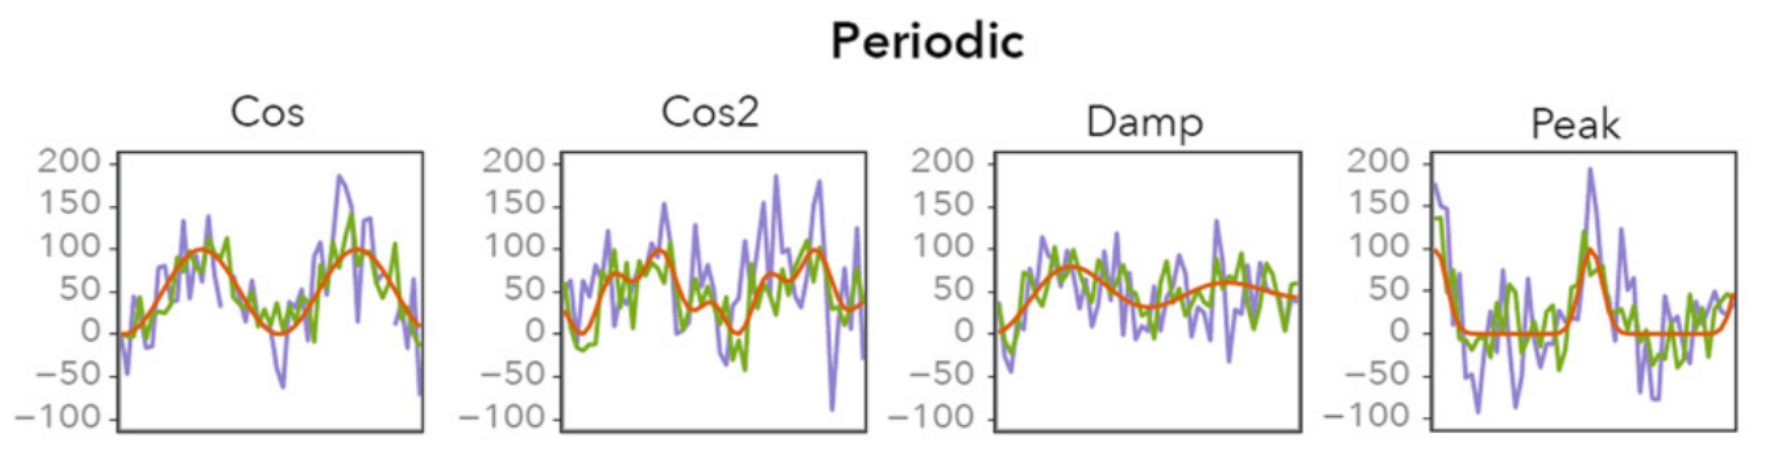
\includegraphics[width=0.9\textwidth]{periodic_time_series.png}
  \caption{Príklad periodických časových radov~\cite{Perea2015}.}
  \label{fig:periodic-time-series}
\end{figure}

\begin{figure}[H]
  \centering
  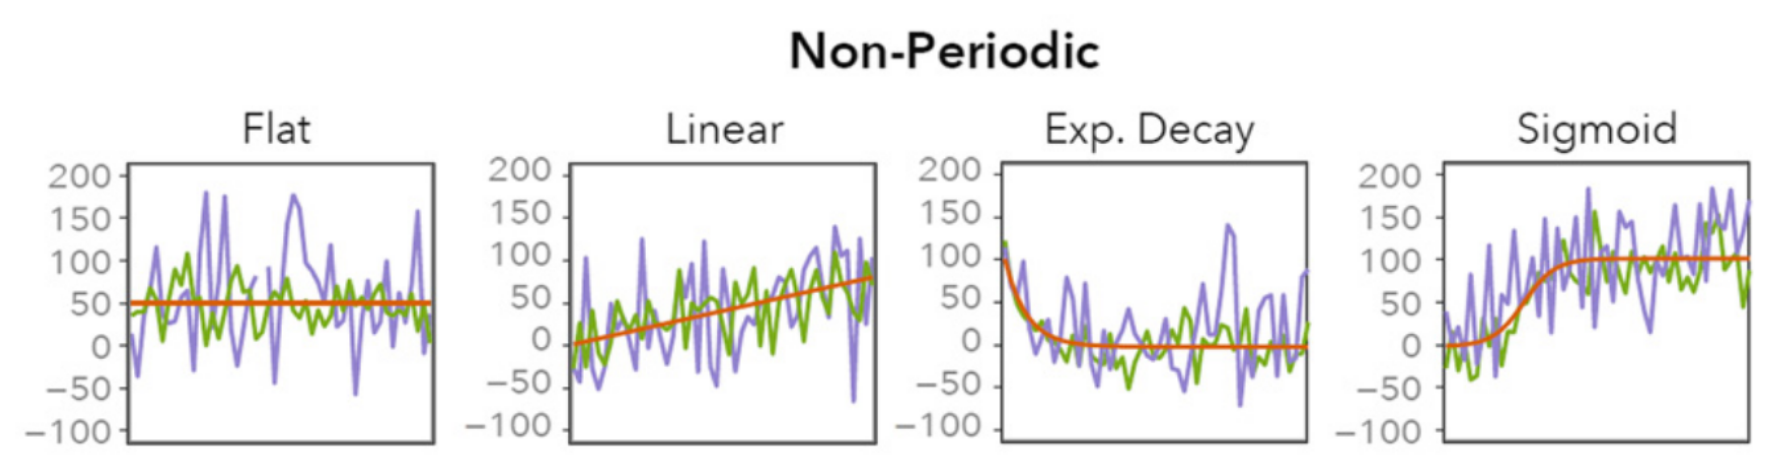
\includegraphics[width=0.9\textwidth]{non_periodic_time_series.png}
  \caption{Príklad neperiodických časových radov~\cite{Perea2015}.}
  \label{fig:non-periodic-time-series}
\end{figure}

%-------------------------------------------------------------------------------
%   Anomaly detection
%-------------------------------------------------------------------------------

\subsection{Detekcia anomálií}
Anomálne správanie alebo anomália je definovaná ako vzor v~správaní, ktorý
nezodpovedá štandardnému správaniu. Pri dátach z~inteligentných meračov,
anomália zodpovedá meraniu, ktoré sa nenachádza v~oblasti normálnych dát.

Pri identifikácii anomálií je najskôr potrebné zamyslieť sa nad nasledovnými
problémami~\cite{Chandola2009}:
\begin{description}
	\item[$\bullet$ Definovanie oblasti normálnych dát] je veľmi náročné, nakoľko
	hranica medzi normálnymi dátami a~anomáliami je nepresná a~môže tak dôjsť
	k~nesprávnemu označeniu meraní.
	\item[$\bullet$ Anomálie vytvorené škodlivou činnosťou] sa javia ako normálne
	dáta, čo sťažuje definíciu normálneho správania.
	\item[$\bullet$ Evolúcia dát] spôsobuje, že definícia normálneho správania sa
	môže časom zmeniť.
	\item[$\bullet$ Presná predstava o anomálii] je často rôzna naprieč viacerými
	odbormi, a~preto neexistuje univerzálny spôsob na určovanie anomálií.
	\item[$\bullet$ Dostupnosť označených dát] zlepšuje presnosť identifikácie
	anomálií, avšak často takéto dáta neexistujú alebo ich je potrebné označiť,
	čo spravidla býva drahé.
	\item[$\bullet$ Biely šum] vyskytujúci sa v~dátach má tendenciu skresľovať
	normálne dáta, ktorých identifikácia je následne zložitá.
\end{description}

Na detekciu anomálií sú používané aj algoritmy určené na klasifikáciu, ako je
napríklad naivný Bayesovský klasifikátor (angl. \textit{Naive Bayes}),
k-najbližší susedia (angl. \textit{k-nearest neighbors}), rozhodovacie stromy
(angl. \textit{decision tree}), náhodné lesy (angl. \textit{random forests}),
neurónové siete so spätnou propagáciou (angl. \textit{neural networks with
backpropagation}) alebo metóda podporných vektorov (angl. \textit{support vector
machine})~\cite{Coma-Puig2016}.

%-------------------------------------------------------------------------------
%   Types of anomalies
%-------------------------------------------------------------------------------

\subsubsection{Typy anomálií}
Dôležitým aspektom pri uplatnení detekcie anomálií je charakter anomálie.
Z~tohto dôvodu môžeme anomálie rozdeliť do nasledujúcich troch skupín.

\paragraph{Bodové anomálie} predstavujú inštancie, ktoré sa nenachádzajú
v~oblasti normálnych dát a~je možné ich detegovať jednotlivo. Jedná sa
o~najjednoduchší typ anomálie a~sústreďuje sa naň väčšina výskumov. Príkladom zo
skutočného života môže byť detekcia podvodov s~kreditnými kartami, kedy
transakcia výrazne väčšieho objemu peňazí predstavuje podvod, zatiaľ čo ostatné
transakcie, nachádzajúce sa v~normálnom rozsahu predstavujú normálne dáta, ktoré
nie sú anomáliou~\cite{Chandola2009}.

\begin{figure}[htbp]
  \centering
  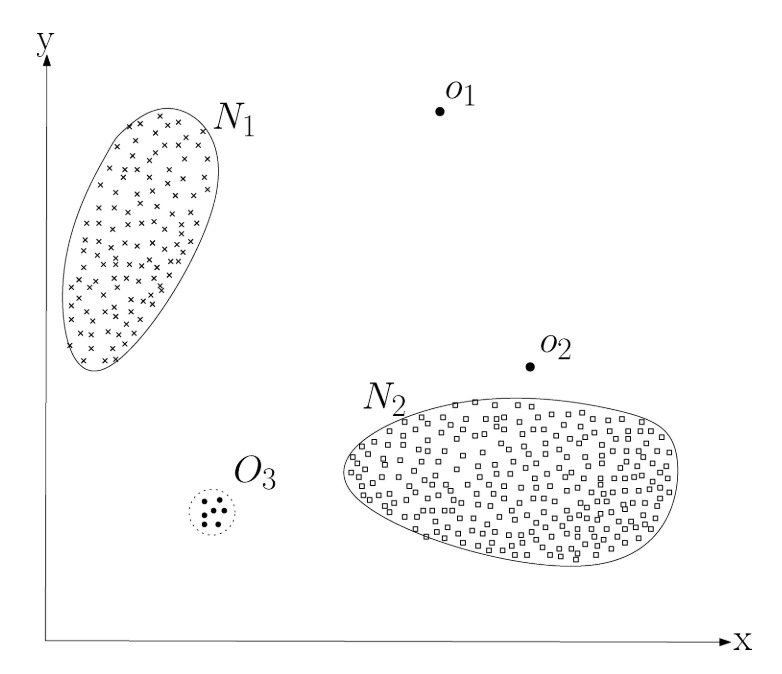
\includegraphics[width=0.9\textwidth]{point_anomalies.png}
  \caption{Príklad bodových anomálií~\cite{Chandola2009}.}
  \label{fig:point-anomalies}
\end{figure}

\paragraph{Kontextové anomálie} predstavujú inštancie, ktoré sa nachádzajú
v~oblasti normálnych dát, ale v~špecifickom kontexte sú považované za anomáliu.
Kontext je daný kontextovými atribútmi v~dátach, na základe ktorých sa určujú
susedné inštancie. Nekontextové atribúty, nazývané aj behaviorálne, reprezentujú
meranú veličinu. Napríklad pri meteorologických meraniach, budú informácie
o~polohe alebo nadmorskej výške predstavovať kontextové atribúty, zatiaľ čo
množstvo zrážok alebo slnečných hodín budú behaviorálne
atribúty~\cite{Chandola2009}.

Anomálne správanie inštancií je dané behaviorálnymi atribútmi v~určitom kontexte.
Čiže ak inštancia s~danými behaviorálnymi atribútmi je považovaná za normálnu,
iná inštancia s~rovnakými behaviorálnymi, ale s~rôznymi kontextovými atribútmi
môže byť považovaná za anomáliu. Kontextové anomálie boli najčastejšie
identifikované v~časových radoch. Príkladom môžu byť opäť transakcie väčšieho
objemu peňazí, ktoré sú bežné v~období pred Vianocami, ale neštandardné v~inom
ročnom období~\cite{Chandola2009}.

Zatiaľ čo v~niektorých prípadoch je definovanie kontextu priamočiare, existujú
domény, kde to jednoduché nie je. Dôležité je aby kontextové atribúty boli
zmysluplne určené v~cieľovej doméne ich aplikácie~\cite{Chandola2009}.

\begin{figure}[htbp]
  \centering
  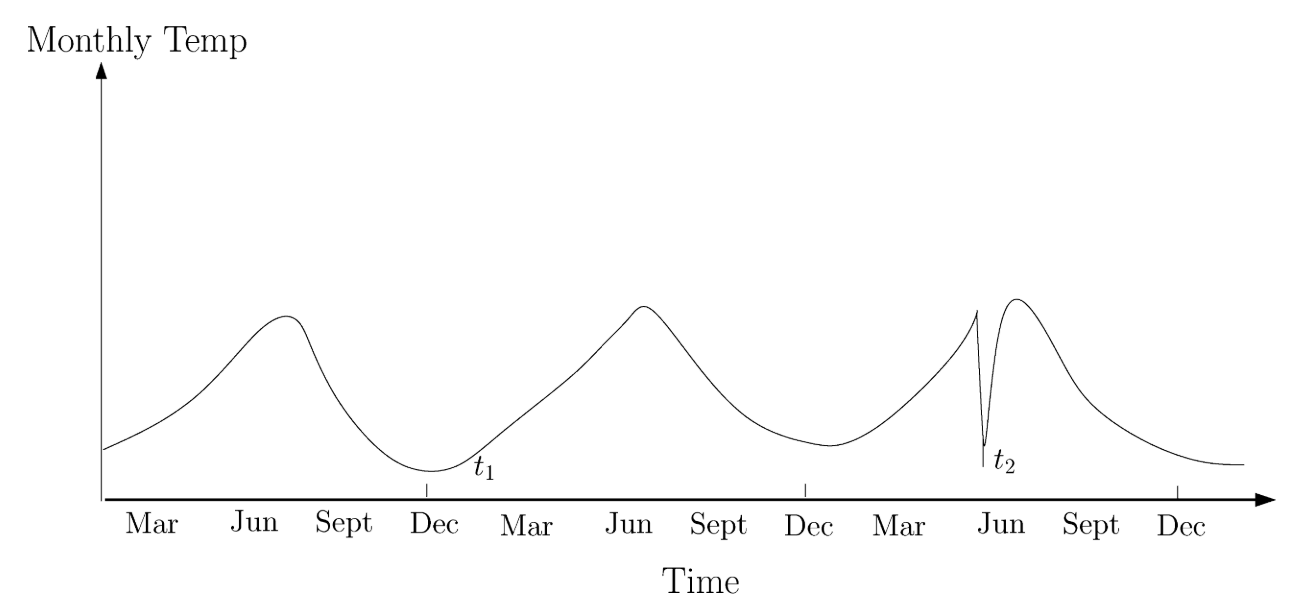
\includegraphics[width=0.9\textwidth]{contextual_anomalies.png}
  \caption{Príklad kontextových anomálií~\cite{Chandola2009}.}
  \label{fig:contextual-anomalies}
\end{figure}

\paragraph{Skupinové anomálie} sa nachádzajú v~oblasti normálnych dát, ale
skupina týchto inštancií tvorí spolu anomáliu. Vzniknutá anomália obsahuje
sekvenciu inštancií, ktorá by pri inom zoradení nepredstavovala anomáliu.
Taktiež sa jednotlivé inštancie môžu nachádzať v~rozsahu normálnych dát.
Príkladom môžu byť systémové volania operačného systému, ktoré sú v~prípade
dodržania určitej postupnosti označené ako činnosť škodlivého
softvéru~\cite{Chandola2009}.

\begin{figure}[H]
  \centering
  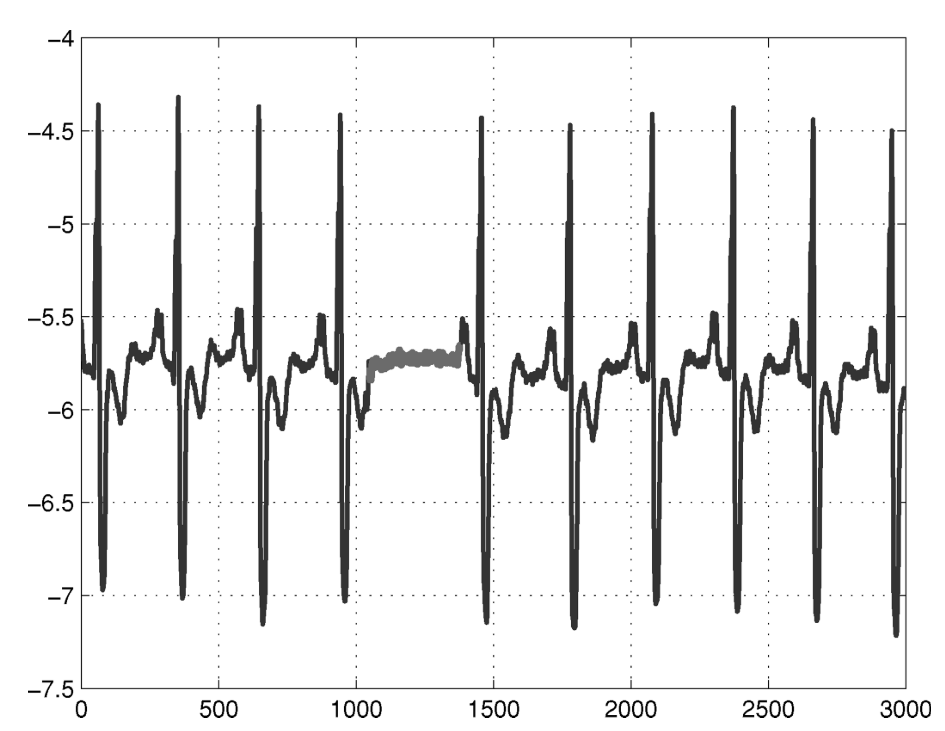
\includegraphics[width=0.9\textwidth]{collective_anomalies.png}
  \caption{Príklad skupinových anomálií~\cite{Chandola2009}.}
  \label{fig:collective-anomalies}
\end{figure}

\noindent
Zatiaľ čo bodové anomálie sa môžu vyskytovať v~každom datasete, skupinové sa
vyskytujú iba v~datasetoch, kde existuje medzi inštanciami vzťah. Pri
kontextových anomáliách je potrebné určiť kontextové atribúty, ktoré sa
v~niektorých datasetoch ani nemusia nachádzať. Problém detekcie bodových
a~skupinových anomálií je možné transformovať na problém detekcie kontextových
anomálií, v~prípade, že sa prihliada na kontext jednotlivých inštancií. Techniky
používané pri detekcii skupinových anomálií sa značne líšia od techník
používaných pri bodových a~kontextových anomáliách~\cite{Chandola2009}.

%-------------------------------------------------------------------------------
%   Range of occurrences anomalies
%-------------------------------------------------------------------------------

\subsubsection{Rozsah výskytu anomálií}
Za anomáliu v~našej doméne považujeme správanie odberateľa, ktoré sa výrazne
líši od ostatných odberateľov. Anomáliou môže byť celé pozorované obdobie alebo
iba jeho určitá časť. Keďže datasety, ktoré máme k~dispozícií obsahujú konečný
počet meraní a~teda nie sú spojité, anomália môže byť reprezentovaná aj jediným
meraním. Anomálie môžme taktiež rozdeliť na pozitívne a~negatívne, v~závislosti
od toho, aké sú očakávané a~reálne hodnoty. Ak je ich rozdiel kladný budeme
hovoriť o~pozitívnych anomáliách, inak o~negatívnych~\cite{Kejariwal2015}.

Intervaly jednotlivých časových radov, ktoré metóda označí ako anomálne, môžeme
ďalej rozdeliť na lokálne a~globálne anomálie. Delenie vzniká na základe
dekompozície časových radov, kde globálne anomálie sú porovnávané so
sezónnou zložkou a~lokálne anomálie sú identifikované vnútri sezónnych vzorov.
Zatiaľ čo globálne anomálie sú identifikované zväčša na základe porovnávania
očakávaných a~reálnych hodnôt, identifikácia lokálnych anomálií je náročnejšia
ak má byť navrhované riešenie robustné. Opäť vychádzame z~porovnávania
očakávaných a~reálnych hodnôt, no jedná sa o~menšie intervaly, ktorých sa môže
vyskytovať rádovo viac. Robustné riešenie to musí zohľadniť a~identifikovať iba
signifikantné anomálie~\cite{Kejariwal2015}.

%-------------------------------------------------------------------------------
%   Anomaly detection approaches
%-------------------------------------------------------------------------------

\subsubsection{Prístupy k identifikácii anomálií}
V praxi sa stretávame s~datasetmi, ktoré sa líšia v~množstve označených dát,
počte typov anomálií, ktoré budeme detegovať alebo aj pomerom medzi normálnymi
inštanciami a~tými neštandardnými. Často je označovanie inštancií vykonávané
manuálne ľudskými expertmi drahé a~neefektívne. Taktiež proces spätnej väzby
môže byť zdĺhavý a~nepraktický. Z~toho dôvodu je dôležité zvoliť správny
prístup pri identifikácií anomálií. V~súčasnosti existujú 3~prístupy, a~to
detekcia anomálií s~učiteľom (angl. \textit{supervised learning}), bez učiteľa
(angl. \textit{unsupervised learning}) a~ich kombinácia (angl.
\textit{semi-supervised learning})~\cite{Chandola2009}.

\paragraph{Detekcia bez učiteľa} nepotrebuje označené trénovacie dáta, vďaka
čomu je široko aplikovateľná a~často používaná. Vychádza z~predpokladu, že
normálne inštancie majú majoritné zastúpenie v~množine. Ak táto podmienka nie je
splnená, môže často dochádzať k~falošnému alarmu~\cite{Chandola2009}.

\paragraph{Detekcia s učiteľom} potrebuje trénovacie dáta s~označenými
inštanciami ako normálnymi, tak aj anomálnymi. Cieľom je vytvoriť prediktívny
model, ktorého úlohou je určiť triedu inštancie. Problémom je nepomer anomálnych
inštancií v~porovnaní s~normálnymi a~ich označenie ľudským expertom môže byť
časovo a~finančne náročné~\cite{Chandola2009}.

\paragraph{Kombinované učenie} je kombináciou predchádzajúcich dvoch prístupov
a~počíta s~označenou iba jednou triedou inštancií. Typicky sú označené normálne
inštancie, keďže ich identifikácia je menej náročná. V~takom prípade je
vytvorený model pre normálnu triedu a~identifikácia anomálií prebieha
v~testovacej vzorke dát~\cite{Chandola2009}.

%-------------------------------------------------------------------------------
%   Anomaly detection techniques
%-------------------------------------------------------------------------------

\subsection{Techniky detekcie anomálií}
\label{c:analysis-techniques}
Detegovať anomálie rôznych typov môžeme niekoľkými spôsobmi, čo závisí aj od
samotných dát. Ich úplnosť, množstvo a~oblasť, v~ktorej boli zozbierané sú
kritické pre správny výber techniky, pomocou ktorej budú anomálie
identifikované. Nás budú zaujímať najmä detekcie anomálií v~časových radoch.
Popísané metódy sú najmä z~oblasti strojového učenia a~dátovej analýzy, ale pre
úplnosť sú spomenuté aj iné používané metódy.

\subsubsection{Klasifikácia}
Pomocou naučeného modelu, nazývaného aj klasifikátor, sú rozoznávané triedy
jednotlivých inštancií. Pri detekcii anomálneho správania, klasifikátor
rozlišuje iba medzi dvoma triedami, triedou normálnych dát a~anomálií. Vzhľadom
na to, že na natrénovanie klasifikátora sú potrebné označené dáta, ide o~učenie
s~učiteľom. Na implementovanie klasifikátora môžeme použiť techniky založené na
rôznych typoch neurónových sietí, Bayesových sieťach, pravidlových systémoch či
metóde podporných vektorov~\cite{Chandola2009,Tan2005}.

\subsubsection{Analýza najbližšieho suseda}
Metóda určí na základe vzdialenosti alebo podobnosti medzi dátovými inštanciami,
či sa jedná o~normálnu inštanciu alebo anomáliu. To je vypočítané pomocou
vzdialeností medzi testovanou inštanciou a~všetkými bodmi, alebo iba \textit{k}
najbližšími bodmi. Pri viacrozmerných dátach je vzdialenosť určovaná pre
každú dimenziu zvlášť. Metóda je založená na predpoklade, že zatiaľ čo normálne
inštancie sa nachádzajú pri sebe a~sú husto usporiadané, anomálie sú
vzdialenejšie, prípadne na okraji vzniknutých oblastí. Aplikácia je možná
pomocou techník založených na relatívnej hustote alebo vzdialenosti najbližších
\textit{k}~susedných inštancií~\cite{Chandola2009,Tan2005}.

\subsubsection{Zhlukovanie}
\label{c:clustering}
Jedná sa o~učenie bez učiteľa, keďže zhluky inštancií sú vytvorené na základe
ich vzdialenosti či podobnosti. Techniky ďalej delíme do kategórií na základe
predpokladu o~dátových inštanciách~\cite{Chandola2009,Tan2005}.

Prvá kategória predpokladá, že normálne inštancie patria do zhluku, zatiaľ čo
anomálne nepatria do žiadneho. Používané sú zhlukovacie algoritmy ako DBSCAN
alebo ROCK, pri ktorých nie nutne každá inštancia musí patriť do zhluku.
Nevýhodou algoritmov môže byť neoptimálne použitie pri detekcií
anomálií, keďže sú primárne určené na riešenie zhlukovacích
problémov~\cite{Chandola2009}.

Druhá kategória predpokladá, že normálne inštancie ležia v~blízkosti
najbližšieho centroidu a~anomálne inštancie sú od neho vzdialené. Algoritmy
väčšinou pozostávajú z~dvoch krokov, v~prvom sú inštancie pridelené do zhluku
a~v~druhom je vypočítané ich anomálne skóre na základe vzdialenosti od centroidu
daného zhluku. Používanými algoritmami sú neurónové siete (konkrétne SOM) alebo
algoritmus k-means, ktoré sa môžu natrénovať aj pomocou kombinovaného učenia. Do
rovnakej skupiny spadá aj metóda k-medoids, ktorá funguje podobne ako k-means,
rozdielom je výpočet centroidov. Pri metóde k-medoids je centroidom inštancia,
ktorej vzdialenosť od všetkých ostatných inštancií je minimálna. Pri k-means
centroidom nemusí byť reálna inštancia~\cite{Chandola2009}.

Posledná kategória pracuje s~predpokladom, že normálne inštancie sú súčasťou
veľkých a~hustých zhlukov, na druhej strane anomálie patria do malých a~riedkych
zhlukov. Používanými algoritmami sú napr. CBLOF
(angl. \textit{Cluster-Based Local Outlier Factor}) alebo \textit{k-d}~stromy.
V~princípe algoritmy najskôr vytvárajú zhluky a~až potom určujú, na základe ich
hustoty, či sa jedná o~normálne zhluky alebo anomálie. Zhluk je vytvorený iba
v~prípade, že inštancia sa nachádza mimo preddefinovaného rádiusu od centra
daného zhluku~\cite{Salvador2005}.

\subsubsection{Štatistické metódy}
Jedná sa o~súbor metód založených na štatistike. K~jednotlivým výpočtom sú
väčšinou používané priemerné hodnoty, odchýlky, atď. V~praxi sa používajú
metódy kĺzavého priemeru, $3\cdot\sigma$ pravidlo, dekompozícia časových radov,
ale aj metóda extrémnej Studentovej odchýlky, ktorá je bližšie opísaná
v~nasledujúcej podkapitole~\ref{c:esd}. Pravidlo $3\cdot\sigma$ je bežne
používané na identifikáciu globálnych anomálie, ktoré sú detegované po
prekročení trojnásobku hodnoty štandardnej odchýlky. Pri sezónnych anomáliach
tento typ detekcie zlyháva, keďže odchýlka je vypočítaná nad celým pozorovaným
časovým radom. Pri jeho segmentácií je metóda úspešná iba v~prípade, kedy sa
odchýlka nepretržite mení~\cite{Hochenbaum2017}.

Metóda kĺzavého priemeru má niekoľko modifikácií, na základe ovahánia
jednotlivých meraní vzniká napr. metóda kĺzavého priemeru s~exponencionálnym
váhovaním (angl. \textit{exponentially weighted moving average}), skrátene
EWMA. Autori v~práci~\cite{Hochenbaum2017} porovnávali okrem EWMA aj PEWMA
(pravdepodobnostné exponencionálne váhovanie), kde v~kombinácií s~metódou ESD
nedosiahli postačujúce výsledky. Kĺzavý priemer zlyhával pri identifikácií
sezónnych anomálií.

%-------------------------------------------------------------------------------
%   Extreme Studentized Deviation
%-------------------------------------------------------------------------------

\subsubsection{Extrémna Studentova odchýlka}
\label{c:esd}
V~práci budeme používať najmä metódu extrémnej Studentovej odchýlky (angl.
\textit{Extreme Studentized Deviation}) a~jej ďalšie derivácie. Metóda
ESD slúži na detekciu viacerých anomálnych inštancií. Jediným vstupným
parametrom metódy je najväčší možný počet podozrivých inštancií v~danom
datasete. Generalizovaná ESD sa snaží maximalizovať odchýlku datasetu
$|x_i - \tilde{x}|$ pre $s$ inštancií. Počet inštancií, sa postupne znižuje,
pokiaľ nie je dosiahnutá stanovená hranica. Pre každý odobraný počet inštancií
sú overované všetky kombinácie. Tento vzťah môžeme zapísať jednoduchou
rovnicou~\ref{eq:gesd} definovanú pre $i$ odobraných inštancií, ktorá je
v~štatistike často označovaná aj ako Grubbov test~\cite{Kuppusamy2013,Rosner1983}.

\begin{equation}
	\label{eq:gesd}
  R_i = \frac
  {max_i |x_i - \tilde{x}|}
  {n - i}
\end{equation}

Do rovnakej kategórie môžeme zaradiť aj sezónnu ESD (angl. \textit{Seasonal
Extreme Studentized Deviation}), ktorá rovnako využíva ESD na identifikáciu
anomálií. Kľúčovým rozdielom je aplikovanie ESD až na dáta, ktoré boli
dekomponované pomocou modifikovaného STL algoritmu. Vďaka tomu algoritmus
deteguje globálne anomálie, ktoré sa rozpínajú mimo očakávaných sezónnych
extrémov, ale aj lokálne anomálie, ktoré by inak ostali zamaskované sezónnou
zložkou časových radov. Modifikácia STL algoritmu pozostáva v~zamenení trendovej
zložky mediánom daného časového radu. Reziduálna zložka je potom vypočítaná ako
rozdiel nameranej hodnoty a~súčtu sezónneho komponentu a~mediánu. Zmena vzorca
použitého na dekompozíciu, zabráni tvorbe falošných anomálií v~reziduálnej
zložke časového radu. Hlavnými obmedzením S-ESD sú datasety obsahujúce
väčšií podiel anomálií. Môžeme si to všimnúť na
obrázku~\ref{fig:sesd-anomalies}, kde anomálie nachádzajúce sa vo zvíraznenom
regióne nie sú detegované, keďže ich množstvo ovplyvňuje ako priemer tak aj
štandardnú odchýlku. Kvôli tomu algoritmus neoznačuje podozrivé pozorovania čím
vzniká mnoho falošne neoznačených inštancií~\cite{Hochenbaum2017}.

\begin{figure}[htbp]
  \centering
  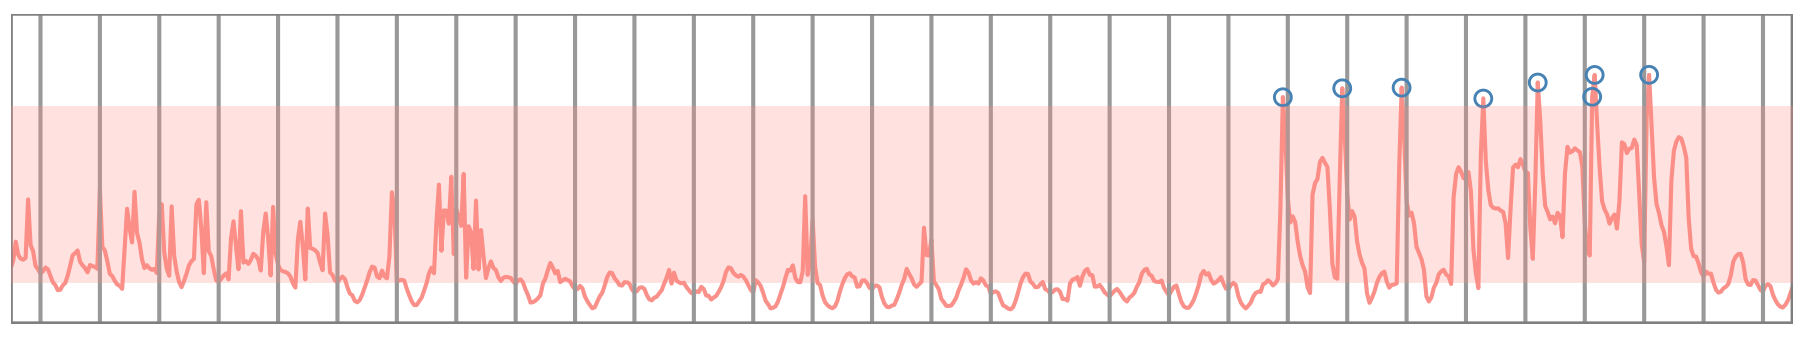
\includegraphics[width=\textwidth]{sesd_anomalies.png}
  \caption{Anomálie detegované pomocou S-ESD algoritmu~\cite{Hochenbaum2017}.}
  \label{fig:sesd-anomalies}
\end{figure}

Cieľom sezónnej hybridnej ESD (angl. \textit{Seasonal Hybrid Extreme
Studentized Deviation}) odstrániť obmedzenia, ktoré vznikajú pri S-ESD.
Rovnako je použitá modifikovaná dekompozícia STL. Rozdiel je v~ESD, kde
namiesto priemeru a~štandardnej odchýlky je použitá robustnejšia štatistická
metóda, ktorá je schopná tolerovať až 50\% anomálií v~časovom rade. Jedná sa
o~absolútnu odchýlku mediánu MAD (angl. \textit{Median Absolute Deviation}),
ktorú vypočítame pomocou vzorca~\ref{eq:mad}~\cite{Hochenbaum2017}.

\begin{equation}
	\label{eq:mad}
  MAD = median_i(|X_i - median_j(X_j)|)
\end{equation}

\noindent
Cenou za to je vyššia výpočtová náročnosť metódy, keďže MAD požaduje zoradenie
dát pred výpočtom ESD. Na druhej strane sú hodnoty F-skóre takmer až o~30\%
vyššie. V~datasetoch s~nízkym počtom výskytov anomálií môže byť vhodnejšie
použitie metódy S-ESD~\cite{Hochenbaum2017}.

\begin{figure}[htbp]
  \centering
  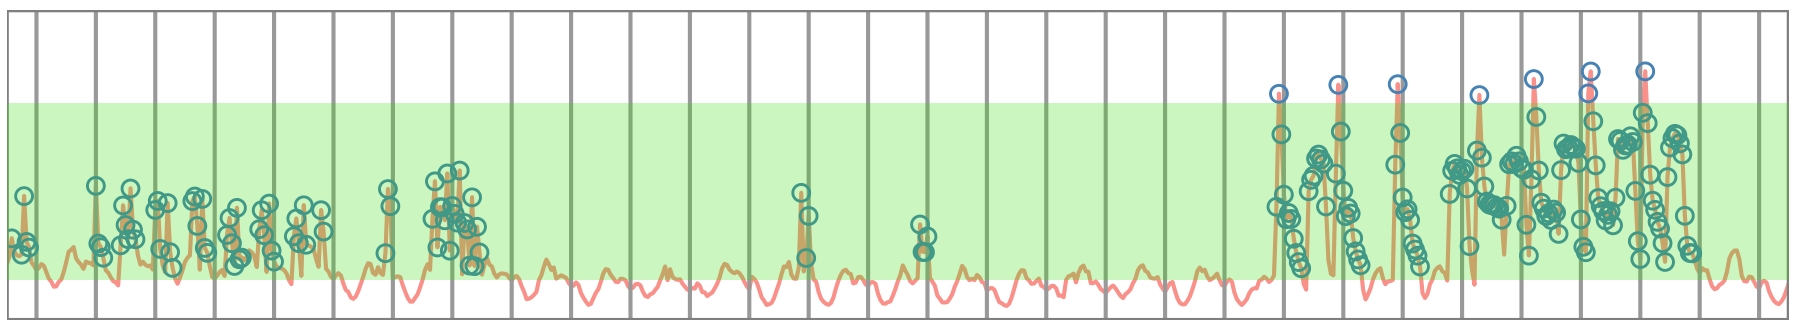
\includegraphics[width=\textwidth]{shesd_anomalies.png}
  \caption{Anomálie detegované pomocou S-H-ESD algoritmu~\cite{Hochenbaum2017}.}
  \label{fig:shesd-anomalies}
\end{figure}

Daľšou metódou založenou na ESD je aj rozšírená S-H-ESD (angl. \textit{Enhanced
Seasonal Hybrid Extreme Studentized Deviation}), ktorej proces pozostáva z~troch
krokov, a~to transformácia dát, dekompozícia časových radov a~analýza
reziduálnej zložky. Účelom transformácie dát je minimalizovať počet falošne
identifikovaných normálnych inštancií a~zároveň normalizovať vstupné časové
rady pomocou Box-Coxovej transformácie, keďže parametrické štatistické testy
dosahujú lepšie výsledky pri normálnom rozdelení dát. Na optimálne nastavenie
parametrov normalizačnej funkcie je použitá metóda maximálnej pravdepodobnosti
(angl. \textit{Maximum Likelihood method}), ktorá je výpočtovo nenáročná
a~vhodná na daný problém. V~procese dekompozície je použitá LOESS regresia
(angl. \textit{Locally Estimated Scatterplot Smoothing}), kedže klasická
dekompozícia môže byť ovplyvnená výskytom anomálií vo vstupných dátach.
Cieľom modifikovanej dekompozície je pomocou série vnorených cykloch a~váh,
robustne a~iteratívne identifikovať trend a~sezónnosť v~danom časovom rade.
Posledným procesom je samotná analýza reziduálnej zložky, kde bežná ESD metóda
potrebuje $k$ ako vstupný parameter označujúci počet anomálnych inštancií.
V~navrhovanej metóde je parameter vypočítaný automaticky na základe štandardnej
odchýlky spracovávaného okna~\cite{Vieira2018}.

%-------------------------------------------------------------------------------
%   Time series classification
%-------------------------------------------------------------------------------

\subsection{Metódy zhlukovania časových radov}
Cieľom zhlukovania je rozdeliť dátové inštancie do \textit{k}~zhlukov na základe
spoločných čŕt. V~prípade, že inštancie sú reprezentované nízkodimenzionálnym
vektorom v~Euklidovom priestore, môžu byť na zhlukovanie použité klasické
techniky spomenuté v~\ref{c:analysis-techniques}. Ak inštancie reprezentujú
časový rad, nasadenie takýchto štandardných prístupov je
zriedkavé~\cite{Hautamaki2008}.

Metódy používané na zhlukovanie časových radov môžeme rozdeliť do 3~skupín, na
základe reprezentácie dát, s~ktorými pracujú. Prvá skupina predpokladá surové
dáta, druhá pracuje s~extrahovanými vlastnosťami z~dát a~posledná metóda
pristupuje k~dátam pomocou vytvoreného modelu. Prístupy sú opísané
v~nasledujúcich podkapitolách~\ref{c:raw-data-clustering},
\ref{c:feature-clustering}, \ref{c:model-clustering}
a~\ref{c:other-clustering}~\cite{Rani2012}.

\subsubsection{Zhlukovanie na základe dočasnej susednosti}
\label{c:raw-data-clustering}
Metóda (angl. \textit{Temporal-Proximity based clustering approach}) pracuje
priamo so surovými, neupravenými dátami, kvôli čomu sa zvykne nazývať aj
zhlukovanie na základe surových dát (angl. \textit{Raw data based clustering
approach}). Hlavným princípom je striedanie viacerých vzdialenostných alebo
podobnostných metrík pre použité časové rady~\cite{Rani2012}.

\label{c:hierarchical-clustering}
\paragraph{Hierarchické zhlukovanie} produkuje vnorenú hierarchiu skupín
podobných časových radov na základe vzdialenostných matíc jednotlivých
inštancií. Hierarchia je graficky reprezentovaná pomocou dendrogramu, príkladom
môže byť graf~\ref{fig:hierarchical-clustering}. Výhodou je, že nie je nutné
zadávať počet zhlukov, ktoré ideme identifikovať. Nevýhodou je obmedzenie
výpočtu iba na menšie datasety, keďže výpočtová zložitosť tejto metódy je
kvadratická~\cite{Dzeroski2007}.

\begin{figure}[htbp]
  \centering
  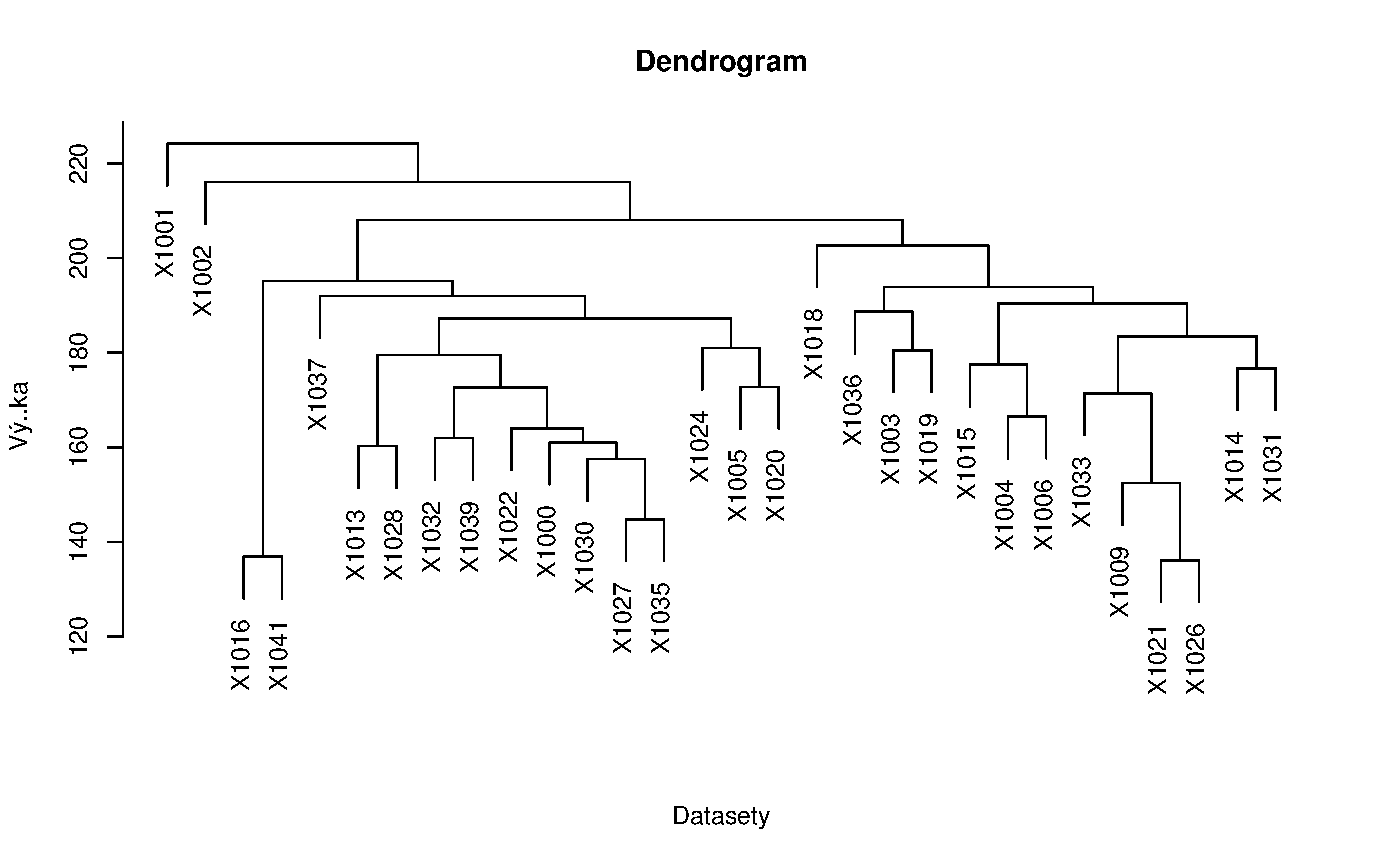
\includegraphics[width=0.95\textwidth]{hierarchical_clustering.pdf}
  \caption{Príklad reprezentácie vytvorených zhlukov pomocou dendrogramu.}
  \label{fig:hierarchical-clustering}
\end{figure}

Metóda hierarchického zhlukovania zoskupuje časové rady do stromu zhlukov. Vo
všeobecnosti existujú dva typy týchto metód, aglomeratívne a~deliace.
Aglomeratívne metódy zo začiatku umiestňujú časové rady do samostatného zhluku,
následne ich postupne spájajú do väčších zhlukov, pokiaľ neexistuje jediný
zhluk, alebo nie je ukončovacou podmienkou práve $k$ zhlukov. Deliace metódy sú
pravým opakom, kedy sú jednotlivé zhluky postupne delené na menšie
a~umiestňované do hierarchického stromu. Na zlepšenie kvality zhlukovania pri
hierarchickom zhlukovaní sú používané bežné zhlukovacie
techniky~\cite{WarrenLiao2005}.

\paragraph{Aglomeratívne zhlukovanie} na základe vzdialenosti medzi dvoma
zhlukmi nameranej pomocou dvojice najbližších časových radov umiestnených
v~rôznych zhlukoch, predstavujú potenciálnych kandidátov na zlúčenie. Podobnosť
môže určovať aj \textit{Wardov algoritmus minimálnej variancie}, ktorý zlúči
zhluky s~najmenším nárastom variancie. V~každom kroku sú tak vyskúšané všetky
kombinácie dvojíc zhlukov, následne je vybrané minimum. Porovnávané časové rady
nemusia mať vždy rovnakú dĺžku. Nevýhodou metódy je najmä vysoký počet operácií,
ale aj neschopnosť spätne zmeniť rozhodnutie zlúčiť
zhluky~\cite{WarrenLiao2005}.

\paragraph{Deliace zhlukovanie} nie je obmedzené iba na časové rady rovnakej
dĺžky. Zároveň tiež nie je možné zmeniť delenie zhluku, ktoré už bolo vykonané.
Na meranie vzdialenosti môžu byť použité metriky opísané
v~\ref{c:distance-metrics}~\cite{WarrenLiao2005}.

\subsubsection{Zhlukovanie na základe reprezentácie}
\label{c:feature-clustering}
Keďže manipulácia so surovými dátami je často náročná a~dáta navyše obsahujú
nadbytočné informácie, táto metóda (angl. \textit{Representation based
clustering approach}) najskôr transformuje dáta do vektoru vlastností a~až
následne sú aplikované zhlukovacie algoritmy. V~literatúre sa zvykne označovať
aj ako zhlukovanie na základe vlastností (angl. \textit{Feature based clustering
approach})~\cite{Rani2012}.

\paragraph{Samoorganizované mapy} predstavujú triedu neurónových sietí, kde
sú neuróny usporiadané v~nízkodimenzionálnej štruktúre. Trénovanie prebieha
iiteratívne a~bez učiteľa. Proces začína pridelením náhodných hodnôt váhovým
vektorom $w$. Každá iterácia trénovania pozostáva z~3~krokov a~to náhodného
výberu vstupného vektoru z~trénovacej množiny, evaluácie siete a~aktualizovaní
váhových vektorov. Po natrénovaní je vypočítaná Euklidova vzdialenosť medzi
vstupným vzorom a~váhovým vektorom. Následne je neurón s~najmenšou vzdialenosťou
označený ako $t$ a~ostatné váhy ostatných neurónov sú aktualizované v~závislosti
od vzdialenosti od neuróna $t$. Nevýhodou je opäť náročné spracovanie časových
radov rôznych dĺžok, keďže dĺžka časového radu definuje aj dĺžku váhového
vektora $w$~\cite{Kohonen2001,WarrenLiao2005}.

\subsubsection{Zhlukovanie na základe modelu}
\label{c:model-clustering}
Metóda (angl. \textit{Model based clustering approach}) predpokladá, že každý
časový rad je generovaný nejakým modelom alebo pravdepodobnostnou distribúciou.
Časové rady sú považované za podobné ak aj modely charakterizujúce jednotlivé
časové rady sú si podobné~\cite{Rani2012}.

\paragraph{ARIMA} model navrhnutý v~práci~\cite{Xiong2002} zhlukuje
jednorozmerné časové rady. Predpokladali, že časové rady sú vygenerované $k$
rôznymi ARIMA modelmi. Vylepšili algoritmus na maximalizáciu očakávaní (angl.
\textit{expectation maximalization algorithm}) tak, že sa naučil správne určiť
koeficienty a~parametre jednotlivých modelov zvyšovaním počtu modelov až do
momentu, kedy vznikol redundantný model. Algoritmus skonvergoval v~prípade, že
počet modelov nebol väčší ako aktuálny počet zhlukov. Na záver boli odstránené
podobné modely, čím sa ešte zmenšil výsledný počet zhlukov $k$.

\subsubsection{Ďalšie prístupy k~zhlukovaniu}
\label{c:other-clustering}
Ďalší prístup je založený na oknách fixnej veľkosti (angl. \textit{Windows based
clustering approach}). V~diskretizovaných časových radoch sú následne
identifikované anomálne úseky. Nevýhodou metódy je náročnosť voľby správnej
veľkosti okna tak, aby zachytila anomáliu a~jej výpočtová
zložitosť~\cite{Teng2010}.

Prístup založený na skrytých Markovovych modeloch (angl. \textit{Hidden Markov
models based approach}) je reprezentovaný výkonným konečným stavovým strojom.
Vychádza z~predpokladu, že existuje skrytý proces, ktorý je Markovský a~zároveň
generuje normálne časové rady. Nevýhodou je, že technika zlyháva v~prípade, že
takýto proces neexistuje. Na základe vytvoreného Markovovho modelu sú merania,
skupina meraní alebo celý časový rad označené za anomálie~\cite{Teng2010}.

%-------------------------------------------------------------------------------
%   Distance metrics
%-------------------------------------------------------------------------------

\subsubsection{Metriky vzdialenosti}
\label{c:distance-metrics}
Kľúčovou záležitosťou pri zhlukovaní časových radov na základe ich podobnosti,
je meranie vzdialenosti medzi nimi. Rovnako ako pri zhlukovaní bodových
inštancií je potrebné definovať si metódy merania vzdialenosti. Najčastejšími
metrikami sú Euklidova a~Manhattanova vzdialenosť. Vhodnosť aplikovania
týchto klasických metód je nízka, keďže nameraná vzdialenosť zachytáva aj
použitú škálu v~dátach. Pri porovnávaní časových radov nás spravidla zaujíma
zmena krivky časového radu a~rovnaká dĺžka porovnávaných časových
radov~\cite{Dzeroski2007,WarrenLiao2005}.

% TODO explain different approaches add figure from real dataset
Metódy používané na meranie vzdialenosti medzi časovými radmi môžeme rozdeliť do
3~skupín založených na atribútoch, na modeloch a~na tvare krivky. Pri
atribútových metódach je pre každý časový rad vypočítaný atribútový vektor, na
základe ktorého je vypočítaná napr. Euklidova vzdialenosť medzi jednotlivými
inštanciami. Modelové techniky používajú parametrický model, do ktorého vstupujú
časové rady. Vzdialenosť je potom definovaná ako vzdialenosť medzi jednotlivými
modelmi. Metódy porovnávajúce tvary kriviek sa snažia prispôsobiť výsledný tvar
časového radu nelineárnym rozťahovaním a~kontrakciou časových
osí~\cite{Hautamaki2008}.


\paragraph{Korelačný koeficient} $r(X, Y)$ meria stupeň lineárnej závislosti
medzi dvoma časovými radmi $X$ a~$Y$. Vyjadríme ho vzorcom~\ref{eq:correlation}.

\begin{equation}
	\label{eq:correlation}
  r \left( X, Y \right) = \frac
  {E \left[ \left( X - E \left[ X \right] \right) \cdot \left( Y - E \left[ Y \right] \right) \right]}
  {E \left[ \left( X - E \left[ X \right] \right)^2 \right] \cdot E \left[ \left( Y - E \left[ Y \right] \right)^2 \right]}
\end{equation}

Korelácia blízka $-1$ znamená, že nárast kriviek časových radov je zrkadlový.
Pri korelácií rovnej $0$ hovoríme o~rozdielnych časových radoch a~pri hodnote
$1$ o~podobných. Na základe hodnoty korelácie, potom môžeme vyjadriť vzdialenosť
vzorcom~\ref{eq:correlation-distance}. Nevýhodou je, ak máme k~dispozícií iba
malú, prípadne krátku časť datasetu. V~takom prípade sa podobnosť touto metrikou
určuje len ťažko. Keďže korelácia zachytáva iba lineárnu podobnosť časových
radov, pri aplikovaní metriky na dva nelineárne podobné časové rady, sú
vyhodnotené ako vzdialené~\cite{Dzeroski2007}.

\begin{equation}
	\label{eq:correlation-distance}
  D_r \left( X, Y \right) = \sqrt{\frac{1}{2} \cdot \left( 1 - r \left( X, Y \right) \right)}
\end{equation}


\paragraph{Dynamické deformovanie času} predstavuje metódu (angl.
\textit{Dynamic Time Warping}), ktorá dokáže zachytiť nelineárne skreslenie
medzi časovými radmi vďaka prideleniu viacerých hodnôt časového radu $X$~druhému
časovému radu $Y$. Takto metóda viac zodpovedá ľudskej intuícii. Na
obrázku~\ref{fig:warping-distance} si môžeme všimnúť, že sú porovnávané hodnoty,
ktoré by sme intuitívne zvolili pri zarovnaní časových radov podľa tvaru krivky.
$D_{DTW}$~je vypočítané pomocou dynamického programovania, práve kvôli množstvu
existujúcich kombinácií. Rekurzia je vyjadrená
vzorcom~\ref{eq:dtw-distance}~\cite{Dzeroski2007,Fu2011,Hsu2015}.
\begin{equation}
	\label{eq:dtw-distance}
  D_{DTW} \left( i, j \right) =
  \begin{cases}
    d \left( x_i, y_j \right) + min
    \begin{cases}
      D_{DTW} \left( i-1, j \right) \\
      D_{DTW} \left( i, j-1 \right) \text{ ak } i \neq 0 \text{ a } j \neq 0  \\
      D_{DTW} \left( i-1, j-1 \right) \\
    \end{cases} \\
    0 \text{ ak } i = 0 \text{ a } j = 0 \\
    \infty \text{ inak}
  \end{cases}
\end{equation}

\begin{figure}[htbp]
  \centering
  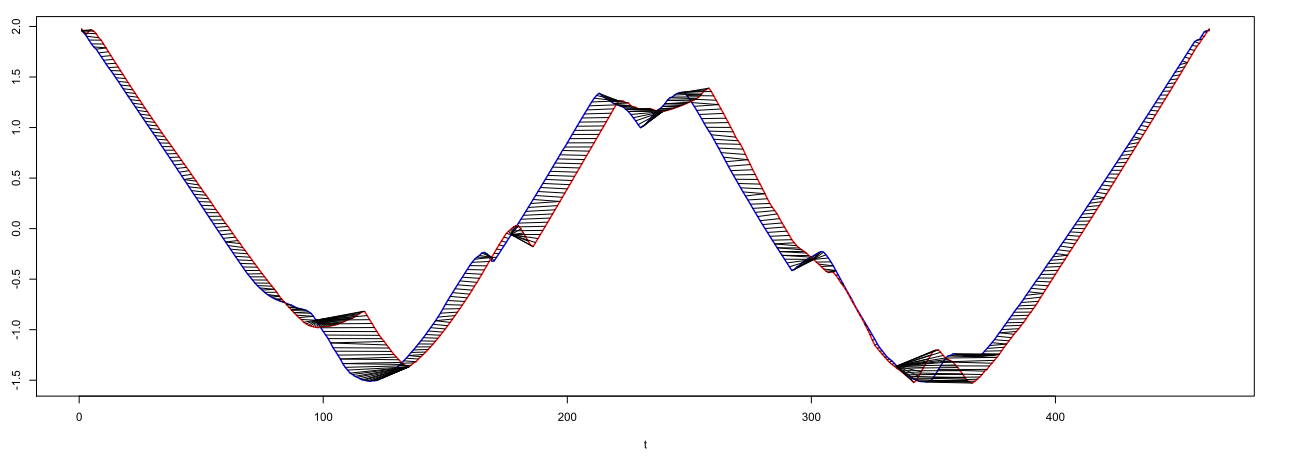
\includegraphics[width=0.95\textwidth]{warping-distance.png}
  % TODO: add missing axis names
  \caption{Príklad porovnávania časových radov pomocou dynamickej deformácií času~\cite{Malinowski2017}.}
  \label{fig:warping-distance}
\end{figure}

\label{c:distance-metrics-gak}
Do rovnakej rodiny vzdialenostných metrík patrí aj rýchle globálne zarovnávanie
kernelov (angl. \textit{Fast global alignment kernels}) skrátene GAK. Cieľom
metódy je znížiť veľkú časovú náročnosť DTW s~dosiahnutím porovnateľných
výsledkov. Podobne aj metrika založená na tvare časových radov (angl.
\textit{Shape-based distance}) skrátene SBD, znižuje časovú náročnosť výpočtu
vzdialenosti medzi časovými radmi. Narozdiel od GAK nepoužíva kernely, ale
štatistické metódy založené na krížovej korelácií (angl.
\textit{cross-correlation}). Bližšie sa týmito metrikami zaoberali autori
v~prácach~\cite{Cuturi2011} a~\cite{Paparrizos2016}.

\paragraph{Kvalitatívna vzdialenosť} je metóda založená na kvalitatívnom
porovnávaní tvaru dvoch časových radov. Pre časové rady $X$~a~$Y$~vyberieme
dvojicu bodov $i$~a~$j$,~ktoré označujú zmenu premennej v~danom časovom rade.
Tak vznikajú 3~možnosti, hodnoty v~časovom rade rastú ($X_i < X_j$), nemenia sa
($X_i \approx X_j$) alebo klesajú ($X_i > X_j$). Vzdialenosť potom vyjadríme
vzorcom~\ref{eq:qualitative-distance}, pomocou ktorého spočítame počet zhôd
v~raste časových radov. Práve funkcia $Diff(q_1, q_2)$ vyjadruje rozdiel v~zmene
rastu. Metóda nemá nevýhody, ktoré vznikali pri korelácií, na druhú stranu je
aplikovateľná iba na krátke časové rady bez toho, aby sa dramaticky znížila
kvalita odhadu vzdialenosti. Podobnosť tvarov kriviek je detegovaná aj
v~prípade, kedy neexistuje medzi časovými radmi lineárna alebo nelineárna
závislosť~\cite{Dzeroski2007}.
\begin{equation}
	\label{eq:qualitative-distance}
  D_q \left( X, Y \right) = \sum_{i=1}^{n-1} \sum_{j=i+1}^{n} \frac
  {2 \cdot Diff \left( q \left( X_i, X_j \right), q \left( Y_i, Y_j \right) \right) }
  {N \cdot \left( N - 1 \right)}
\end{equation}

\paragraph{Euklidova vzdialenosť} je používaná najmä pri klasických
zhlukovacích problémoch. Ak zvolený časový rad má dĺžku $n$, vzdialenosť
vypočítame vzorcom~\ref{eq:distance-euclidean}. Na
obrázku~\ref{fig:euclidean-distance} sú vždy porovnávané hodnoty vyskytujúce sa
v~rovnakom čase $t$~\cite{WarrenLiao2005}.
\begin{equation}
	\label{eq:distance-euclidean}
  D_E \left( X, Y \right) = \sqrt{\sum_{k=1}^{n} \left( X_{ik} - Y_{jk} \right)^2 }
\end{equation}

\begin{figure}[htbp]
  \centering
  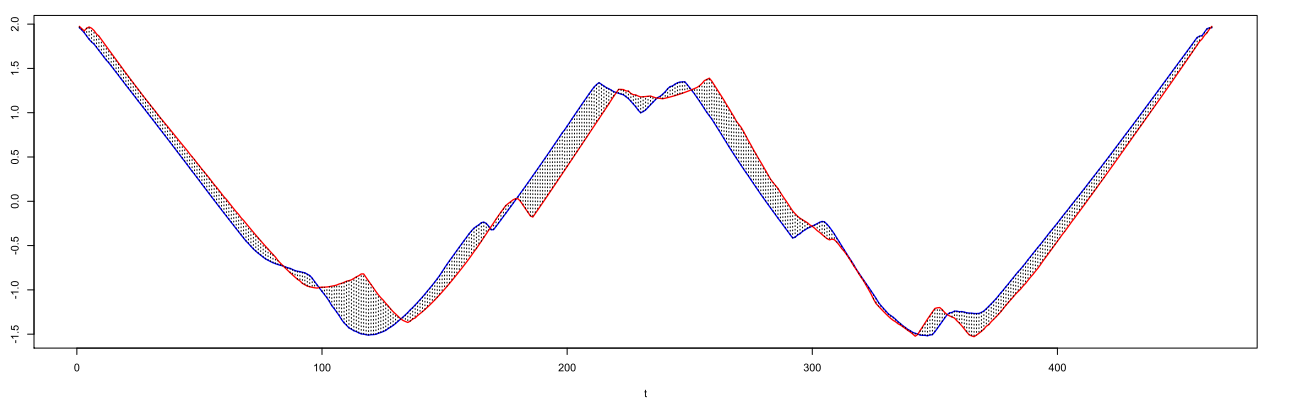
\includegraphics[width=0.95\textwidth]{euclidean-distance.png}
  % TODO: add missing axis names
  \caption{Príklad porovnávania časových radov pomocou Euklidovej vzdialenosti~\cite{Malinowski2017}.}
  \label{fig:euclidean-distance}
\end{figure}

\paragraph{Manhattanovská vzdialenosť} je rovnako ako Euklidova vzdialenosť
používaná najmä pri klasických zhlukovacích problémoch. Výpočet je tiež veľmi
podobný, môžeme ho vyjadriť vzorcom~\ref{eq:distance-manhattan}~\cite{Craw2017}.

\begin{equation}
	\label{eq:distance-manhattan}
  D_M \left( X, Y \right) = \sum_{k=1}^{n} \lvert X_{ik} - Y_{jk} \rvert
\end{equation}

\paragraph{Pearsonov korelačný koeficient} je používaný pri výpočte
vzdialenosti, ktorá je založená na vzájomnej korelácií. Vo
vzorci~\ref{eq:distance-pearson} reprezentuje $\widetilde{X}$~aritmetický
priemer časového radu $X$. Vzdialenosť vyjadríme
vzorcom~\ref{eq:distance-pearson}~\cite{WarrenLiao2005}.
\begin{equation}
	\label{eq:distance-pearson}
  r \left( X, Y \right) = \frac
  { \sum_{i=1}^{n} \left( X_{i} - \widetilde{X} \right) \cdot \left( Y_{i} - \widetilde{Y} \right) }
  { \sqrt{\sum_{i=1}^{n} \left( X_{i} - \widetilde{X} \right)^2 } \cdot \sqrt{\sum_{i=1}^{n} \left( Y_{i} - \widetilde{Y} \right)^2 } }
\end{equation}
\begin{equation}
	\label{eq:distance-golay}
  D_P \left( X, Y \right) = 2 \cdot \left( 1 - r \left( X, Y \right) \right)
\end{equation}

\paragraph{Vzdialenosť medzi krátkymi časovými radmi} je metóda (angl.
\textit{Short time series}), ktorá meria vzdialenosť ako sumu štvorcových
rozdielov medzi krivkami jednotlivých časových radov. Na odstránenie nežiadúcich
efektov škály sa používa \textit{z} štandardizácia. Matematicky vzdialenosť
vyjadríme vzorcom~\ref{eq:sts-distance}. Zložka $t_k$ predstavuje
čas~\cite{WarrenLiao2005}.
\begin{equation}
	\label{eq:sts-distance}
  D_{STS} \left( X, Y \right) = \sqrt{ \sum_{k=1}^{n} \left(
    \frac{Y_{j \left( k+1 \right)} - Y_{jk}}{t_{\left( k+1 \right)} - t_k} -
    \frac{X_{i \left( k+1 \right)} - X_{ik}}{t_{\left( k+1 \right)} - t_k}
   \right)^2 }
\end{equation}

%-------------------------------------------------------------------------------
%   Preprocessing data
%-------------------------------------------------------------------------------

\subsection{Predspracovanie dát}
Pri metódach založených na dátovej analytike a~strojovom určení je nesmierne
dôležité zvoliť vhodnú reprezentáciu dát, vybrať atribúty, ktoré sú relevantné
pre zvolený problém a~často krát aj odstrániť chýbajúce alebo nekompletné časové
rady. Znalosť vstupných dát a~špecifickosť danej domény prináša
k~predspracovaniu dát ďalšie prístupy, ktoré zvyšujú správnosť použitých úprav.

Najčastejšie používanými vysvetľujúcimi premennými sú:
\begin{itemize}
  \item geografická poloha
  \item voltáž distribučnej siete
  \item tarifná skupina
  \item energetická sebestačnosť
  \item pravidelnosť platieb
  \item priemerná spotreba
  \item používané elektrospotrebiče
  \item veľkosť a~typ objektu
\end{itemize}
Ďalšou premennou, ktorá vysvetľuje krátkodobé zmeny v~správaní jednotlivých
odberateľov je počasie. To je pre viacerých odberateľov rovnaké a~viaže sa na
konkrétny región, v ktorom sa nachádza meteorologická stanica. Dáta z~nich sú
väčšinou verejne dostupné~\cite{Stankovic2014}.

\subsubsection{Filtrovanie odberateľov}
Dáta z~inteligentných meračov bývajú často nekompletné a~s~chýbajúcimi
hodnotami. Väčšina algoritmov nedokáže spracovať takéto dáta a~všetky časové
rady musia byť rovnakej dĺžky. Rovnako sú nepoužiteľné dáta, ktoré boli
poškodené pri samotnom zbere dát, nie však pri meraní. Zatiaľ čo chybné meracie
zariadenia môžu spadať do detekcie anomálií a~zaujímajú nás, dáta ktoré boli
zduplikované alebo inak poškodené až pri ukladaní môžeme vylúčiť z~datasetu.
Prípady, kedy zákazník bol zapojený do siete až v~priebehu meraní, musíme
ošetrovať špeciálne, najčastejšie vynechaním alebo orezaním na najbližšiu menšiu
dĺžku posuvného okna~\cite{Nagi2008}.

\subsubsection{Výber atribútov}
Väčšina dát pochádzajúcich z~inteligentných meračov obsahuje iba stĺpce
s~časovou známkou a~momentálnou spotrebou daného uzlu v~sieti. Z~týchto
informácií ešte vieme vyčítať, mesiac, týždeň, deň prípadne deň v~týždni alebo
sviatok. Niektoré z~extrahovaných atribútov úzko súvisia s~funkciou spotreby
elektrickej energie. Pri vytváraní presného modelu je preto nevyhnutné správne
identifikovať takéto atribúty. Otestovanie všetkých kombinácií by bolo časovo
a~výpočtovo náročné. Najjednoduchším spôsobom je vytvorenie korelačnej matice
jednotlivých vysvetľujúcich premenných a~sledovanej veličiny~\cite{Cody2015}.

\subsubsection{Extrakcia čŕt}
Ďalšou technikou používanou pri príprave dát je tvorba nových atribútov
založených na pôvodných, surových dátach. V~súvisiacom článku~\cite{Nagi2008}
ide napr. o~vytvorenie hodinového priemeru pre každého zákazníka. Vzťah
priemernej spotreby $x_h$ môžeme definovať rôzne, v~našom prípade ide o~podiel
mesačnej priemernej spotreby nasledujúceho mesiaca $P_{h+1}$~a~rozdielu dennej
spotreby v~aktuálnom a~nasledujúcom mesiaci $D_{h+1} - D_{h}$, čo zapíšeme
vzorcom~\ref{eq:feature-extraction}.
\begin{equation}
	\label{eq:feature-extraction}
  x_h = \frac{P_{h+1}}{D_{h+1} - D_{h}}
\end{equation}

\subsubsection{Reprezentácia FeaClip}
\label{c:feaclip-representation}
Ako bolo už spomenuté, niektoré datasety obsahujú informácie iba o~meranej
veličine, čo niekedy nemusí byť postačujúce. Preto vznikajú nové atribúty
popisujúce sledovanú veličinu. Jednou z~nich je metóda FeaClip, ktorá
reprezentuje dáta pomocou bitového reťazca, z~ktorého sú vytvorené nové
atribúty. Nad vybraným posuvným oknom nad datasetom je aplikovaná transformácia
popísaná rovnicou~\ref{eq:feaclip}, čím sú merania s~hodnotami väčšími ako
priemer aktuálneho posuvného okna nahradené hodnotou 1, inak 0. Na vzniknutý
reťazec je aplikované kódovanie dĺžky behu (angl. \textit{Run-length
encoding}). Beh je súvislá postupnosť jedného znaku, dĺžka behu predstavuje
počet znakov v~takomto behu. Analyzované okno časového radu je transformované
na osmicu čísel, a~to maximum z~dĺžok jednotkových behov, maximum z~dĺžok
nulových behov, počet jednotiek v~reťazci, počet prechodov medzi rôznymi behmi
a~počty prvých a~posledných núl a~jednotiek. Výhodami reprezentácie sú najmä
redukcia dimenzií, zvýraznenie charakteru dát, paralelizmus a~jednoduchá
interpretácia dát~\cite{Laurinec2018}.

\begin{equation}
  \label{eq:feaclip}
  \hat{x_i} =
  \begin{cases}
    1 \text{ ak } x_i > \mu \\
    0 \text{ inak } \\
  \end{cases}
  \text{, pre i } \in (1, 2, ..., 48)
\end{equation}

\subsubsection{Agregácia dát}
Dáta z~meračov sú dostupné v~pravidelných intervaloch. Pre jednoduchšiu
manipuláciu s~časovými radmi a~redukciu dimenzií, môžu byť dáta agregované do
väčších intervalov. Pri použití viacerých datasetov s~rôznou frekvenciou zberu,
je agregácia hustejšieho časového radu nutná, keďže by tak vzniklo množstvo
chýbajúcich hodnôt. Agregácia dát tiež vyhladzuje malé odchýlky v~časových
radoch, čo môže sťažiť identifikáciu náhlej zmeny správania odberateľov. To môže
viesť k~nesprávnemu označeniu správania odberateľa za
neštandardné~\cite{Cody2015}.

Cieľom agregácie časových radov môže byť aj redukcia na priemer, prípadne
medián, dňa alebo týždňa. So zredukovanými dátami je potom možné pracovať rýchlo
a~efektívne, keďže ich pamäťová náročnosť je iba zlomkom oproti pôvodnej.
Zároveň však vzniká priestor na stratenie informácie o~anomálnej aktivite
odberateľa, čo je nutné zvážiť pri konkrétnej implementácii.

\subsubsection{Redukcia dimenzií}
\label{c:dimension-reduction}
Jednou z~najjednoduchších metód používaných pri redukcii dát je práve
vzorkovanie (angl. \textit{sampling}). Parametrami sú $m$~a~$n$, ktoré
predstavujú počet dimenzií pred a~po procese vzorkovania. Vzdialenosť sa medzi
jednotlivými inštanciami zväčšuje, no zároveň je rovnaká medzi všetkými
inštanciami. Nevýhodou je, že tvar výsledného časového radu je oproti pôvodnému
skreslený, čo môžeme vidieť na obrázkoch~\ref{fig:data-reduction-orig}
a~\ref{fig:data-reduction-agg}~\cite{Fu2011}.

\begin{figure}[htbp]
  \centering
  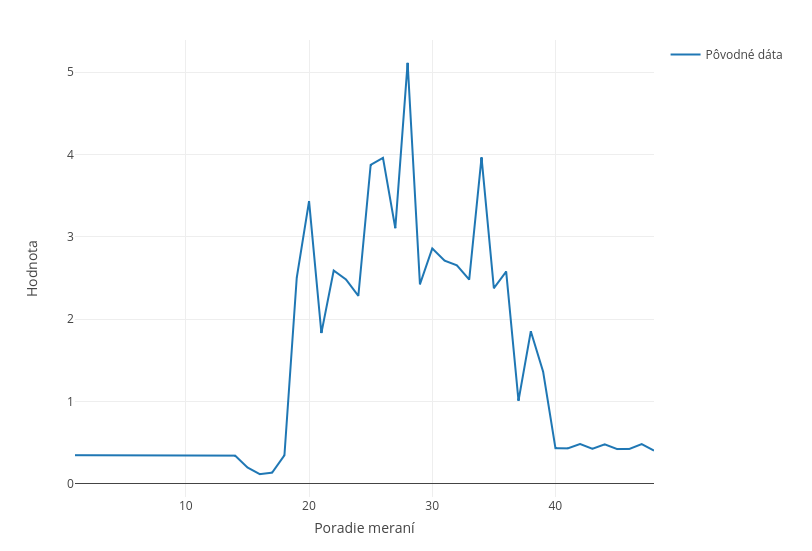
\includegraphics[width=\textwidth]{data_reduction_orig.png}
  \caption{Časový rad bez úprav}
  \label{fig:data-reduction-orig}
\end{figure}

Lepšie výsledky dostaneme ak pri vzorkovaní budeme priemerovať hodnoty vo
vzniknutých intervaloch. Táto metóda sa zvykne nazývať aj po častiach agregovaná
aproximácia (angl. \textit{piecewise aggregate approximation}), skrátene PAA.
Vylepšenou verziou je metóda APCA, kde vzniknuté intervaly majú rôznu dĺžku,
v~závislosti od tvaru časového radu. Taktiež môžeme okrem priemeru použiť medián
zvoleného intervalu. Obe metódy môžeme vidieť na
obrázku~\ref{fig:data-reduction-agg}~\cite{Keogh2002}.

Ďalšou metódou je aproximácia pomocou rovných čiar, kde hlavnými kategóriami sú
lineárna interpolácia a~lineárna regresia. Bežnou metódou pri interpolácií je
použiť po častiach lineárnu aproximáciu (angl. \textit{piecewise linear
approximation}). Algoritmus začína vytvorením odhadu časového radu, ktorý
používa polovicu vytvorených intervalov. Tie sú následne zlučované, pokiaľ nie
je splnené ukončovacie kritérium, napr. celkový počet intervalov. Poradie
zlučovania je určené na základe ceny zlučovania~\cite{Fu2011}.

Žiaducim efektom pri redukovaní dimenzií je zachovanie charakteristických bodov.
Tieto body sa zvyknú nazývať percepčne dôležité body (angl. \textit{perceptually
important points}), skrátene PIP. Algoritmus najskôr určí prvé tri body, a~to
prvý, posledný a~bod, ktorý je od týchto dvoch najvzdialenejší. Ďalšie body sú
určované na základe maximálnej vertikálnej vzdialenosti medzi dvoma susednými
bodmi PIP. Proces pokračuje pokiaľ nie sú zoradené podľa dôležitosti všetky
pôvodné body. Na obrázkoch~\ref{fig:data-reduction-orig}
a~\ref{fig:data-reduction-agg} môžeme vidieť, že tvar kriviek pôvodného časového
radu a~redukovaného je mierne odlišný, čo je spôsobené roztiahnutím alebo
zúžením podintervalov v~redukovanom časovom rade~\cite{Fu2011}.

\begin{figure}[htbp]
  \centering
  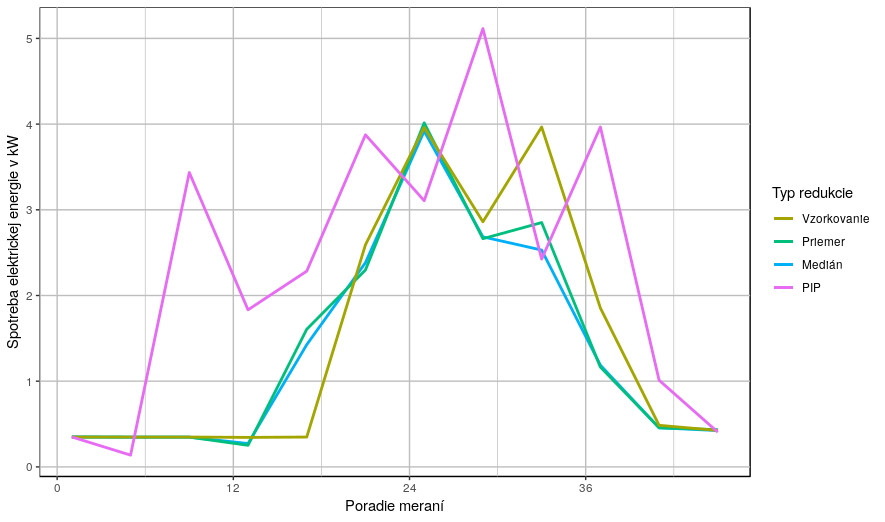
\includegraphics[width=\textwidth]{data_reduction_agg.png}
  \caption{Redukované časové rady}
  \label{fig:data-reduction-agg}
\end{figure}

Ďalší prístup používaný pri reprezentovaní časových radov je ich konvertovanie
z PAA do symbolickej formy. Najskôr sú diskretizované do intervalov, ktoré sú
následne konvertované do symbolov. Táto metóda sa nazýva symbolická agregovaná
aproximácia (angl. \textit{symbolic aggregate approximation}), skrátene SAX.
Algoritmus rozdelí obor hodnôt na regióny a~každý z~nich je namapovaný na iný
symbol~\cite{Fu2011}.

Ďalšou metódou je analýza hlavných komponentov (angl. \textit{principal
component analysis}), skrátene PCA. Obvykle sa PCA používa na elimináciu menej
významných komponentov, čím sa znižuje dimenzionalita dát. Metóda má uplatnenie
aj pri analýze či vizualizácií vysokodimenzionálnych dát~\cite{Fu2011}.
% TODO add something more about PCA and also eq

Na podobnom princípe ako DTW je založené aj hľadanie najdlhšej spoločnej
podpostupnosti (angl. \textit{longest common subsequence}), skrátene LCSS. Ide
o~variáciu editačnej vzdialenosti a~spájania dvoch sekvencií, ktoré sa môžu
natiahnuť a~vynechať tak niektoré elementy bez toho, aby sa menilo ich poradie
v~rámci postupnosti. Narozdiel od DTW, výstupy nie sú skreslené anomáliami
v~dátach~\cite{Fu2011}.

\subsubsection{Segmentácia časových radov}
Časové rady sú charakteristické súvislým priebehom, a~preto pri ich segmentácii
je nutné čeliť viacerým problémom. Najjednoduchším prístupom je rozdeliť časový
rad pomocou okna fixnej dĺžky do segmentov, z~ktorých vznikajú jednoduché vzory.
Jedinou úlohou je správne zvoliť dĺžku okna. Pri použití tejto metódy existujú
dva hlavné problémy. Typické vzory môžu mať variabilnú dĺžku a~ich výskyt môže
byť rôzny. Práve preto je vhodnejšie použiť dynamický prístup, ktorý rozdeľuje
časový rad práve v~bodoch, ktoré zachovávajú cyklicky vyskytujúce sa vzory
a~vznikajú tak segmenty s~rôznymi dĺžkami~\cite{Fu2011}.

\subsubsection{Normalizácia číselných vektorov}
\label{c:z-score}
Rozsahy nameraných hodnôt inteligentnými meračmi sa môžu líšiť, pri jednotlivých
odberateľoch dokonca aj rádovo. Pri zhlukovaní takýchto časových radov je preto
potrebná najskôr ich normalizácia, v~prípade zhlukovania na základe tvaru
priebehov. Existuje viacero druhov normalizácií, no v~práci budeme používať
najmä štandardné skóre, nazývané aj z-skóre (angl. \textit{z-score}). Hodnotu
vypočítame ako podiel rozdielu hodnoty a~priemeru a~štandardnej odchýlky.
Normalizáciu vyjadríme nasledujúcim
vzorcom~\ref{eq:z-score}~\cite{Arampatzis2009}
\begin{equation}
	\label{eq:z-score}
  z = \frac{x-\mu}{\sigma}
\end{equation}

%-------------------------------------------------------------------------------
%   Identification of abnormal behavior
%-------------------------------------------------------------------------------

\subsection{Anomálie v~energetických časových radoch}
V~distribučných sieťach vznikajú straty, ktoré vo všeobecnosti môžeme rozdeliť
na technické a~netechnické. Technické straty sú spôsobené vlastnosťami
obvodu ako napr. odporom materiálu či únikmi cez poškodenú izoláciu a~môžu sa
meniť pri rôznych teplotách či počasí. Medzi netechnické straty patria najmä
nelegálne odbery. V~práci sa budeme zaoberať ich identifikáciou na základe
anomálneho správania spotrebiteľa. Keďže je časovo a~finančne náročné
pravidelne kontrolovať odberateľov tak, aby sa predišlo nelegálnemu odberu,
je potrebné znížiť počet podozrivých odberateľov na minimum a~zároveň
maximalizovať pravdepodobnosť, s~ktorou budú kontrolovaní iba odberatelia
s~neštandardnými odbermi~\cite{Coma-Puig2016,Sahoo2015}.

Pri identifikácií anomálií je spravidla najskôr definovaná oblasť, ktorej
inštancie považujeme za normálne. Za anomálie považujeme inštancie nachádzajúce
sa mimo oblasti, alebo na jej okraji. V~prípade, že na trénovanie modelu máme
k~dispozícií označené iba anomálne dáta, je najskôr definovaná oblasť anomálnych
dát a~až následne normálna oblasť. Pri identifikácií anomálií v~časových radoch
v~doméne energetiky je takýto prístup len ťažko aplikovateľný nakoľko podobné
časové rady pri rôznych domácnostiach môžu, ale nemusia predstavovať normálne
správanie~\cite{Spiric2015}.

Najčastejšími metódami používanými pri nelegálnom odbere je obídenie meračov
spotreby energie či samotná manipulácia s~nimi. Merače tak poskytujú nesprávne
informácie o~spotrebovanej energie odberateľmi, čo je možné detegovať až po
identifikácii celkových netechnických strát v~sieti. Ďalšou populárnou metódou
používanou na detekciu nelegálnych odberov je analýza spotrebiteľského
profilu zákazníka, kedy je našou snahou identifikovať nepravidelné vzory
v~nameraných spotrebiteľských dátach~\cite{Sahoo2015}. Tak ako je spomenuté
v~práci~\cite{Depuru2012}, nelegálne odbery môžu prebiehať iba v~určitom čase
prípadne iba pri zvýšenej spotrebe. Identifikácia takýchto nelegálnych odberov
je náročná a~prípadná kontrola nemusí odhaliť manipuláciu s~meracím zariadením.

Vďaka inteligentným meračom je možné detegovať nelegálne odbery omnoho
rýchlejšie, najmä kvôli vysokej frekvencii zberania údajov. Takto sú
identifikované aj také odbery, ktoré by sa pri klasických meraniach stratili
v~týždenných alebo mesačných agregáciách. Úspešnosť detekcie nelegálnych odberov
je výrazne vyššia najmä pri neštandardných spotrebách alebo ak sa jedná
o~neopakujúcu udalosť. Problém vzniká ak odberateľ systematicky mení
nelegálnu spotrebu a~kopíruje vzory, ktoré vznikajú v~dátach pri legálnom
odbere. Vtedy je potrebné mať k~dispozícií väčšie množstvo dát a~zároveň použiť
zložitejšie algoritmy detekcie anomálií, ktoré sú popísané v~súvisiacej
práci~\cite{Nikovski2013}.

V~súvisiacich prácach sa autori zaoberali určením netechnických strát
v~elektrických distribučných sieťach s~použitím rôznych štatistických metód
alebo strojového učenia. Dostupné dáta od distribútorov pochádzali najmä
z~jedného zdroja, lokality a~zameriavali sa na jeden zdroj energie. Dáta, ktoré
budeme mať k~dispozícií disponujú podobnými vlastnosťami. V~súvisiacej
práci~\cite{Coma-Puig2016} boli použité viaceré zdroje dát a~energie, následkom
čoho bola zvýšená presnosť identifikácie anomálneho správania odberateľa.
Ďalším zdrojom dát môžu byť agregované hodnoty meraní z~klasických meračov,
prípadne spätná väzba zo samotných kontrol odberateľov.

Typickou črtou netechnických strát je negatívny skok v spotrebe elektrickej
energie. Nasleduje po poškodení inteligentného meracieho zariadenia alebo pri
začatí nelegálneho odberu. Pokles môže byť zapríčinený aj zmenou počtu ľudí,
miestností prípadne ich funkcie alebo zvýšením energetickej sebestačnosti.
Následkom je nižšia nameraná spotrebe energie v dlhšom horizonte. Zníženie
spotreby môže byť čiastočné alebo úplné, ako môžeme
vidieť na obrázkoch~\ref{fig:decrease-partial}
a~\ref{fig:decrease-total}~\cite{Spiric2015,Trevizan2015}.

\begin{figure}[htbp]

	\begin{minipage}{0.45\textwidth}
		\begin{center}
			\captionsetup{justification=centering}
			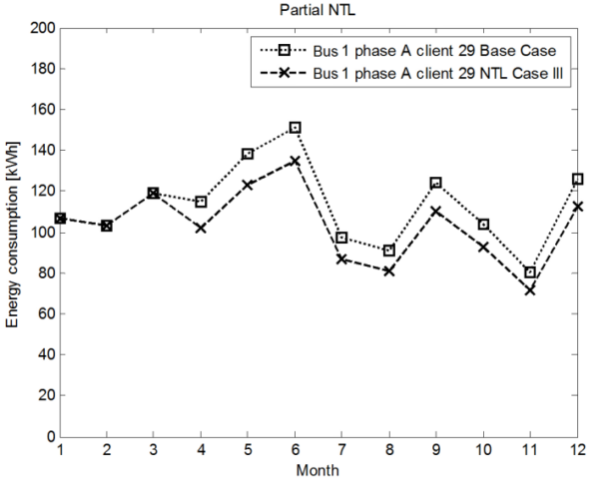
\includegraphics[scale=0.33]{decrease-partial.png}
			\caption{Čiastočné zníženie spotreby elektrickej energie~\cite{Trevizan2015}.}
			\label{fig:decrease-partial}
		\end{center}
	\end{minipage}
  \centering
  \begin{minipage}{0.45\textwidth}
    \begin{center}
      \captionsetup{justification=centering}
      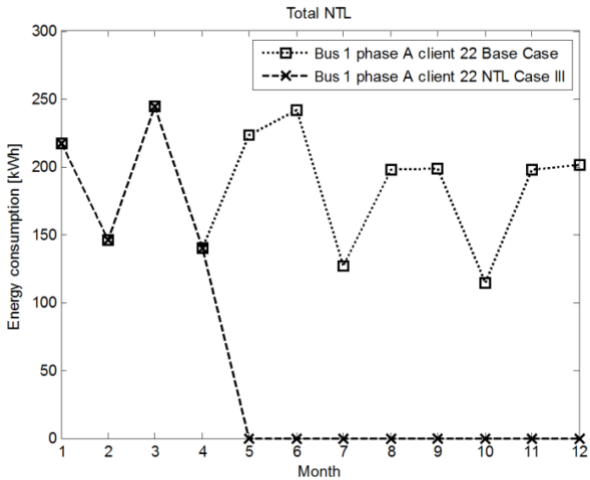
\includegraphics[scale=0.33]{decrease-total.png}
			\caption{Úplné zníženie spotreby elektrickej energie~\cite{Trevizan2015}.}
			\label{fig:decrease-total}
    \end{center}
  \end{minipage}\hfill

\end{figure}

Z~pohľadu výskytu anomálie môžu nastať nasledovné scenáre:
\begin{itemize}
  \item Anomália vznikne neodborným pripojením odberateľa do energetickej siete alebo existuje ešte pred tým ako, nastane zber dát inteligentnými meračmi.
        Keďže celý časový rad pozostáva z~chybných dát, odhalenie anomálie je nepravdepodobné.
  \item Anomália vznikne v~priebehu sledovaného intervalu a~zároveň je odhalená a~ďalej sa už nevyskytuje.
  \item Anomália vznikne v~priebehu sledovaného intervalu a~nie je odhalená. Táto skupina je predmetom celej našej práce.
\end{itemize}
Prvý prípad anomálií je možné odhaliť iba na základe vysvetľujúcich premenných,
ktoré nemusia byť pravdivé, ak sú dodané samotným odberateľom. Druhú skupinu je
potrebné v~dátach označiť, prípadne anomálne merania vynechať pri ďalšom
klasifikovaní~\cite{Spiric2015}.

%-------------------------------------------------------------------------------
%   Evaluation metrics
%-------------------------------------------------------------------------------

\subsection{Vyhodnocovacie metriky}
\label{c:evaluation-metrics}
Za predpokladu, že získané dáta budú obsahovať aj označené inštancie, prípadne
budú označené dodatočne na základe výpočtov, môžeme na vyhodnotenie úspešnosti
použiť aj maticu zámen. V~takom prípade budeme musieť predpovedať triedu
jednotlivých inštancií, a~teda či sa jedná o~normálneho alebo anomálneho
odberateľa. Jednoduchý klasifikátor označí prvých \textit{n} odberateľov,
ktorých miera pravdepodobnosti výskytu anomálneho odberu je najvyššia, za
anomálnych. Pri vyjadrení matice zámen pomocou
tabuľky~\ref{tab:confusion-matrix} potom riadky predstavujú predpovedanú triedu
a~stĺpce skutočnú. Vznikajú tak 4~kategórie, správne označení podozriví
odberatelia (angl. \textit{true positive}), nesprávne označení podozriví
odberatelia (angl. \textit{false positive}), nesprávne označení normálni
odberatelia (angl. \textit{true negative}) a~správne označení normálni
odberatelia (angl. \textit{false negative}). Kvalitu klasifikácie potom môžeme
zmerať pomocou presnosti a~pokrytia. Presnosť vypočítame
vzorcom~\ref{eq:precision}, kedy ide o~pomer správne označených anomálií
a~celkový počet označených anomálií. Tým vypočítame percento odberateľov,
ktorých sme správne klasifikovali ako podozrivých.
\begin{equation}
	\label{eq:precision}
  \text{Presnosť} = \frac{TP}{TP + FP}
\end{equation}
Pokrytie označuje pomer správne označených anomálií a~celkový počet skutočných
anomálií. Vyjadríme ju pomocou vzorca~\ref{eq:recall}.
\begin{equation}
	\label{eq:recall}
  \text{Pokrytie} = \frac{TP}{TP + FN}
\end{equation}
Aby sa predišlo situácií, kedy sa v~dátach nachádza iba malý počet anomálnych
odberateľov a~pre model by tak bolo výhodnejšie označovať iba tých, s~ktorými si
je takmer istý, je dôležité brať do úvahy aj túto metriku. Obe metriky sú
vyjadrené v~percentách~\cite{Trevizan2015,Wei2006}.

\begin{table}[htbp]
	\centering
	\caption{Matica zámen}
	\label{tab:confusion-matrix}
	\begin{tabular}{|c|c|c|c|}
		\hline
		\multicolumn{2}{|c|}{\multirow{2}{*}{}} 									 & \multicolumn{2}{c|}{skutočnosť} 							 \\ \cline{3-4}
		\multicolumn{2}{|c|}{}       									      			 &  anomálna kategória   &  normálna kategória   \\ \hline
		\multirow{2}{*}[1.2pt]{predikcia}   &  anomálna kategória  &  TP (true positive)   &  FP (false positive)  \\ \cline{2-4}
																				&  normálna kategória  &  FN (false negative)  &  TN (true negative)   \\ \hline
	\end{tabular}
\end{table}

Ďalšou používanou metrikou je aj tzv. F-skóre, ktoré obsahuje informácie oboch
predchádzajúcich metrík. Keďže ide o~súčet metrík, tiež je vyjadrené
v~percentách. Cieľom práce je maximalizovať túto metriku. F-skóre vyjadríme
pomocou vzorca~\ref{eq:f-score}, kde $P$~predstavuje presnosť a~$C$ predstavuje
pokrytie~\cite{Trevizan2015}.
\begin{equation}
	\label{eq:f-score}
  F = 2 \cdot \left( P^{-1} + C^{-1} \right)^{-1}
\end{equation}

\subsubsection{Zhlukovacie validačné indexy}
\label{c:cluster-validity-indeces}
Zhlukovanie je metóda, ktorej cieľom je určiť skupinu, do ktorej spadá daná
inštancia. Triedenia prebieha na základe atribútov inštancie. Keďže sa jedná
o~učenie bez učiteľa, je potrebná validácia výsledného zhlukovania. V~praxi sa
používajú validačné indexy zhlukov (angl. \textit{cluster validity indeces}).
Indexy sa delia na externé a~interné, v~závislosti od dostupnosti skutočných
tried zhlukovaného datasetu~\cite{Arbelaitz2013}.

\paragraph{Externé indexy zhlukov} obsahujú napr. Randov, Jaccardov alebo
Fowlkes-Mallowsov index. Naivným prístupom je porovnávanie zhlukov a~počítanie
dvojíc inštancií, ktoré sa nachádzajú v~rovnakom zhluku. Maticu zámen tak
môžeme prepísať do tabuľky~\ref{tab:validation-matrix}. Časové rady nachádzajúce
sa v~rovnakom zhluku pri rôznych zhlukovaniach \textit{X} a~\textit{Y} sa
nachádzajú v~kategórií \textit{true positive}~\cite{Bilgic2018}.

\begin{table}[htbp]
  % TODO: move to another page or down
	\centering
	\caption{Validačná matica zhlukovania časových radov}
	\label{tab:validation-matrix}
	\begin{tabular}{|c|c|c|}
		\hline
		 																		&  Rovnaké v množine \textit{Y}   &  Rôzne v množine \textit{Y}   \\ \hline
		Rovnaké v množine \textit{X}  			&  TP (true positive)   					&  FP (false positive)  				\\ \hline
		Rôzne v množine \textit{X}  				&  FN (false negative)  					&  TN (true negative)   				\\ \hline
	\end{tabular}
\end{table}

Spomínané validačné indexy môžeme vyjadriť nasledujúcimi vzorcami, a~to Randov
index vzorcom~\ref{eq:rand}, Jaccardov index vzorcom~\ref{eq:jaccard}
a~Fowlkes-Mallowsov index vzorcom~\ref{eq:fowlkes}. Indexy sú bližšie popísané
v~práci~\cite{Bilgic2018}.

\begin{equation}
	\label{eq:rand}
  \text{RI} = \frac{TP}{FP + FN + TP}
\end{equation}
\begin{equation}
	\label{eq:jaccard}
  \text{J} = \frac{TP + TN}{FP + FN + TP + TN}
\end{equation}
\begin{equation}
	\label{eq:fowlkes}
  \text{FM} = \frac{TP}{\sqrt{(TP + FP)(TP + FN)}}
\end{equation}

\paragraph{Interné indexy zhlukov} predstavujú jedinú metriku, ktorou je možné
overiť zhlukovanie pri dátach, ktoré neobsahujú skutočné triedy inštancií. Medzi
používané indexy patria napr. Dunnov index, Calinski-Harabasov index, Gamma
index, C-index, Davies-Bouldinov index, Silhouetteov index a~mnoho ďalších.
V~práci~\cite{Arbelaitz2013} autori analyzovali a~porovnali 30 rôznych
validačných indexov na rôznych datasetoch. Na syntetických datasetoch sa najviac
osvedčili Silhouetteov index, modifikovaný Davies-Bouldinov index
a~Calinski-Harabasov index. Pri reálnych datasetoch boli výsledky podobné, čiže
indexy s~horšími výsledkami dosiahnutými pri syntetických datasetoch ich
dosahovali aj na reálnych dátach. Vyššie spomenuté 3 indexy dosiahli však horšie
skóre ako skórovacia funkcia, generalizované Dunnove indexy a~COP index.

\begin{figure}[htbp]
  \centering
  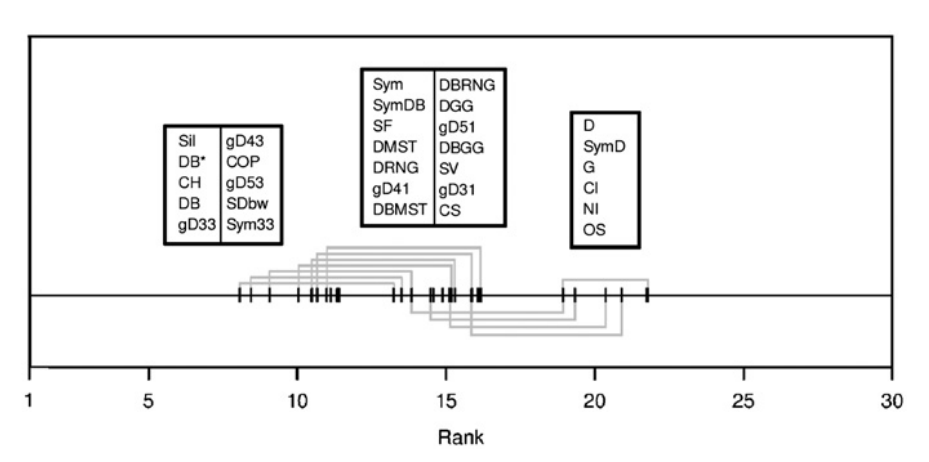
\includegraphics[width=0.8\textwidth]{shaffer_test.png}
  \caption{Výsledky Shafferovho testu so stupňom dôležitosti 10\%~\cite{Arbelaitz2013}.}
  \label{fig:shaffer-test}
\end{figure}

V~závere autori vyhodnotili výsledky svojich experimentov a~graficky ich
interpretovali pomocou Shafferovho testu~\ref{fig:shaffer-test}. Nižší rank
predstavuje lepšie výsledky validačného indexu na rôznych datasoch. Zároveň
neexistuje výrazný štatistický rozdiel medzi jednotlivými indexami
nachádzajúcich sa v~rovnakej skupine. Aj keď nie je možné jednoznačne určiť
objektívne najlepší validačný index, autori odporúčajú indexy nachádzajúce sa
v~prvej skupine indexov a~to napr. Silhouetteov index, modifikovaný
Davies-Bouldinov index, Calinski-Harabasov index,  Davies-Bouldinov index,
generalizovaný Dunnov index a~COP index~\cite{Arbelaitz2013}.

%-------------------------------------------------------------------------------
%   Related work
%-------------------------------------------------------------------------------

\subsection{Súvisiace práce v~doméne energetiky a~indentifikácií anomálií}
V~\cite{Hautamaki2008} bola pri zhlukovaní použitá aj kombinácia viacerých
metód, konkrétne k-means, metóda náhodnej výmeny a~aglomeratívne zhlukovanie.
Ako už bolo spomenuté v~\ref{c:analysis-techniques}, úlohou algoritmu k-means
namapovať existujúce inštancie do \textit{k} zhlukov. Aj keď metóda náhodnej
výmeny je obmedzená na zhlukovacie problémy v~Euklidovom priestore, bola
použitá aj pri zhlukovaní časových radov a~zabraňuje zaseknutiu zhluku
v~lokálnom minime. V~princípe je náhodne vybraný zhluk, ktorý bude vymazaný a~za
centroid bude vybraný jeden časový rad z~neho. Ak takéto riešenie je lepšie ako
bez rozpustenia zhluku je nahradené pôvodným. Ako bolo spomenuté
v~\ref{c:hierarchical-clustering}, cieľom aglomeratívneho zhlukovania je všetky
časové rady označiť ako zhluky a~následne ich iteratívne zhlukovať. V~momente,
keď je vytvorených \textit{k} zhlukov, je vypočítaný centroid zhluku a~určená
hierarchia zhlukov.
\medskip

\noindent
V~práci~\cite{Cody2015} boli pri určovaní podozrivých aktivít odberateľov
úspešne aplikované rozhodovacie stromy. Po vytvorení trénovacej a~testovacej
množiny boli vygenerované rozhodovacie pravidlá reprezentujúce model normálnej
spotreby elektrickej energie. Po predikcii boli porovnané predikované
a~testovacie dáta pomocou štatistickej metódy RMSE. Výsledkom experimentov je
dostatočne presná predikcia spotreby energie, vypočítaná iba na základe
atribútov extrahovaných z~časovej známky. Prekročením stanovej hranice boli
inštancie považované za anomálne. Počas experimentov boli použité M5P
rozhodovacie učiace stromy.
\medskip

\noindent
Predmetom článku~\cite{Tagaris2002} bolo navrhnúť novú vlnovú techniku na
reprezentovanie viacerých vlastností meraných dát. Tiež vytvorili nový model,
ktorý v~sebe zahŕňa viacero modelov, čím je pridávanie ďalších komponentov do
detekčného systému jednoduché. Navrhovaná metóda je citlivá na lokálne zmeny vo
vzore dát. Taktiež dosiahli s~relatívne malým množstvom meraní presnosť až 78\%
na trénovacej množine a~70\% na testovacej množine. Metóda je citlivá na zmeny
amplitúd a~frekvencií v~dátach z~meračov. Nevýhodou je, že model nie je citlivý
na nevýrazné zmeny a~trendy v~dátach.
\medskip

%-------------------------------------------------------------------------------
%   Analysis evaluation
%-------------------------------------------------------------------------------

\subsection{Zhodnotenie analýzy}
Narastajúce množstvo zbieraných dát v~doméne energetiky z~monitorovaných
systémov predstavuje množstvo skrytých znalostí. Vzniká potreba vydolovať ich
a~následne využiť na optimalizáciu procesov, zníženie prevádzkových nákladov
alebo predpovedanie budúcej záťaže energetických sietí. Na základe
nepredvídateľných udalostí alebo náhodného správania odberateľov vznikajú
v~datasetoch intervaly, ktoré nezodpovedajú štandardnému správaniu. Tie
označujeme ako intervaly s~výskytom anomálií. Cieľom našej práce ich bude nájsť
a~zmenšiť dĺžku nájdeného intervalu tak, aby bol čo najmenší, no zároveň v~sebe
zahŕňal identifikované anomálie.

Identifikácia anomálií v~časových radoch prináša so sebou viacero výziev, medzi
tie najčastejšie patrí vysoká dimenzionalita dát, definícia normálneho správania,
ale najmä absencia označených dát. Označenie dát je navyše náročné pre ľudského
experta a~taktiež sa veľmi líši definícia anomálie pri rôznych doménach. Ani
normálne správanie nie je možné jednoznačne a~jednoducho určiť, keďže tisíce
odberateľov sa správa unikátne. Z~dostupných dát však vieme po normalizácií
extrahovať vzory, ktoré po následnom zhlukovaní predstavujú rádovo menej skupín,
s~ktorými ďalej pracujeme ako s~definíciou normálneho správania. Väčšina článkov
zaoberajúca sa zhlukovaním, sa zameriava na nízkorozmerné dáta. Pri
vysokodimenzionálnych dátach sú metriky podobnosti inštancií zväčša zamerané na
tvary jednotlivých priebehov, než na absolútne hodnoty pozorovaní.

Cieľom našej práce je pomocou zhlukovania časových radov vhodne zadefinovať
normálne správanie odberateľov a~presnejšie identifikovať intervaly obsahujúce
anomálie. Pri zhlukovaní časových radov experimentálne overíme vhodnosť voľby
hyperparametrov ako je napr. počet zhlukov, vzdialenostná metrika alebo veľkosť
použitého posuvného okna. Riedke zhluky budeme považovať za anomálne a~budú
podrobené ďalšej analýze, kedy budú identifikované zlomy, lokálne a~globálne
anomálie.

Vzhľadom na to, že dostupné dáta neobsahujú informáciu o~anomáliách, budeme pri
evaluácií riešenia používať syntetický dataset, ktorý bude vytvorený na základe
dostupných dát a~znalostí o~anomáliách.

%-------------------------------------------------------------------------------
%   Chapter 3 - Solution design
%-------------------------------------------------------------------------------

\newpage
\section{Návrh riešenia}
\label{c:solution-design}
Pomocou metód strojového učenia a~dátovej analytiky sa zameriame na
identifikáciu anomálií v~časových radoch v~oblasti distribučných spoločností. Na
základe dostupných dát môžu nastať dva rôzne scenáre. Ak dataset bude obsahovať
iba časovú známku a~spotrebu elektrickej energie daného zákazníka, zhlukovanie
je možné iba na základe časového radu spotreby a~výsledky budú evaluované
pomocou vzdialeností medzi jednotlivými časovými radmi vo vnútri zhlukov.
Naopak, ak dataset obsahuje viaceré vysvetľujúce premenné, potom je možné
vytvoriť model, ktorý bude zhlukovať odberateľov na základe týchto atribútov.
Tak bude zabezpečená evaluácia pôvodného zhlukovacieho modelu. Dáta, ktoré máme
k~dispozícií obsahujú iba časovú známku, množstvo odoberanej elektrickej energie
a~príznak označujúci dni pracovného pokoja.

Z~experimentov môžeme predpokladať, že zhlukovacie algoritmy vytvárajú husté
a~riedke zhluky. Primárne sa budeme zameriavať na analýzu časových radov,
ktoré spadajú do riedkych zhlukov a~už ony samotné môžu predstavovať anomálie.
Cieľom je v~takýchto časových radoch čo najpresnejšie identifikovať
a~lokalizovať intervaly s~neštandardným správaním odberateľa. Musíme pri tom
brať ohľad najmä na cyklus dní a~týždňov, no zároveň pristupovať k~zvykom
odberateľov jednotlivo a~zvážiť ich pri označovaní anomálneho intervalu.

% Zvýšiť presnosť odhaľovania anomálií je možné aj osobitným prístupom
% k~jednotlivým odberateľom. Práve vďaka identifikácií zlomov v~časových radoch je
% možné presnejšie určiť správanie odberateľa. Zároveň algoritmus poskytuje ďalší
% mechanizmus na určovanie intervalu, v~ktorom sa mení správanie odberateľa, ktoré
% môžeme považovať za anomáliu.

Výstupom opísaného procesu sú podozrivé a~anomálne časové rady a~jednotlivé
merania v~nich, ktoré sú taktiež považované za anomálie. Na výstupe sa môže
podieľať viacero algoritmov, čo je potrebné zohľadniť pri vytváraní výsledného
skóre. Na záver je potrebné zlúčiť jednotlivé merania do intervalov, ktoré
svojim skóre opisujú mieru istoty, že označený interval obsahuje anomáliu.
Výhodou takéhoto spracovania je univerzálnosť riešenia, jednoduchá vizualizácia,
ale najmä klasifikácia rôznych typov anomálií. Zatiaľ čo lokálne anomálie sú
výsledkom krátkodobej zmeny správania odberateľa a~môže sa jednať aj o~výsledok
náhody, globálne anomálie predstavujú výraznejšiu alebo dlhodobejšiu zmenu,
ktorá môže byť predmetom záujmu distribútorov elektrickej energie.

Pre lepšie znázornenie je opísaný postup vizualizovaný stavovým diagramom na
obrázku~\ref{fig:state-diagram}. Jednotlivé kroky sú ďalej rozpísané
v~nasledujúcich kapitolách.

\begin{figure}[htbp]
  \centering
  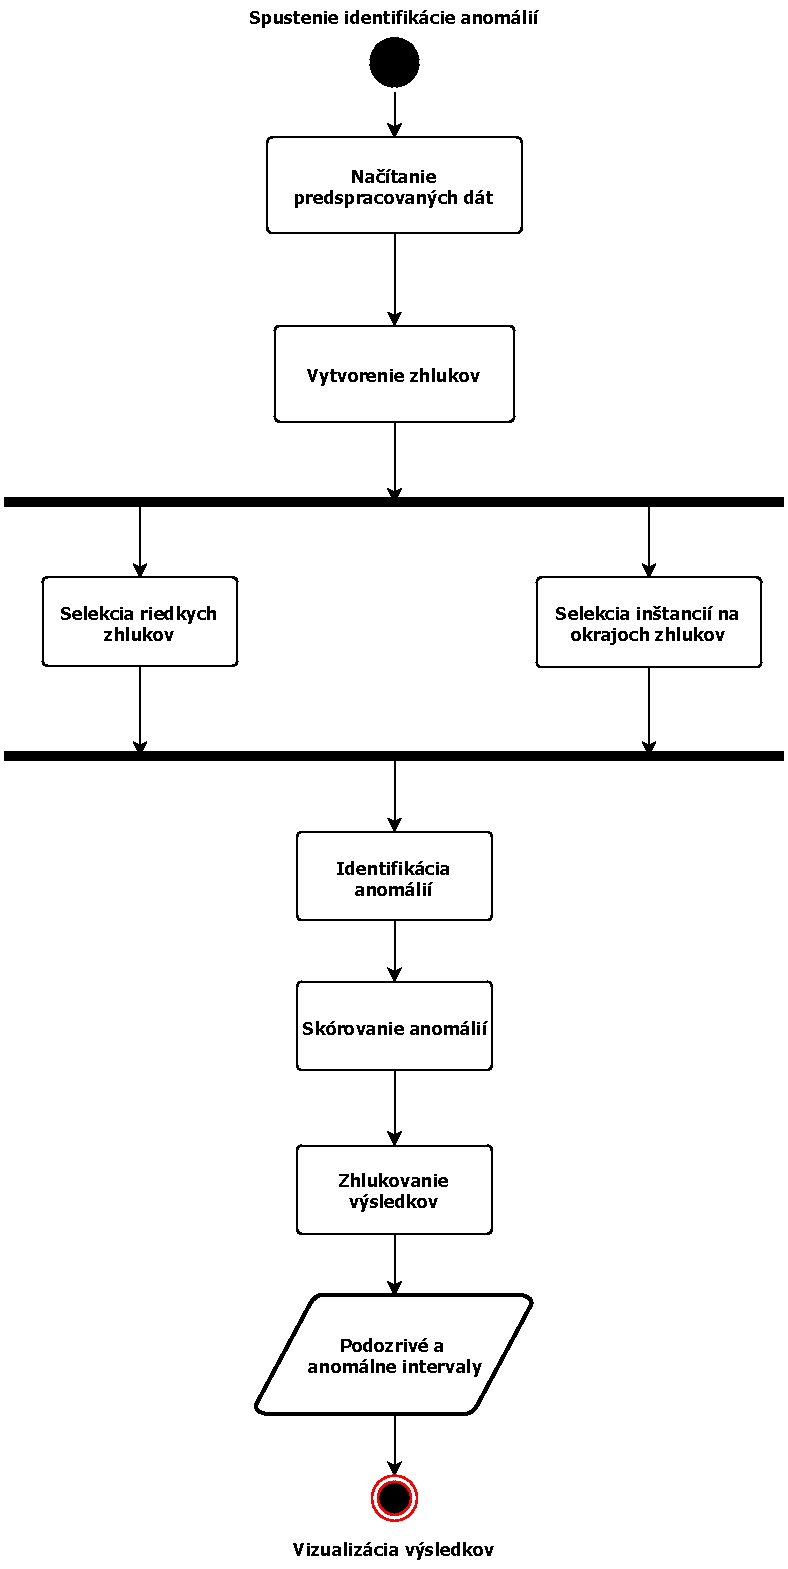
\includegraphics[width=0.65\textwidth]{state_diagram.pdf}
  \caption{Stavový diagram procesu identifikácií anomálií.}
  \label{fig:state-diagram}
\end{figure}

Dáta sú po načítaní rozdelené do dvoch skupín. Prvá skupina obsahuje iba
pracovné dni, druhá víkendy a~sviatky. Cieľom je zachytiť podobné správanie
odberateľov do jednej skupiny tak, aby sa neprekrývalo. Vzniknuté časové rady je
nutné pred ďalším spracovaním normalizovať, napr. pomocou z-skóre. Normalizácia
je potrebná kvôli použitým metrikám podobnosti časových radov, ktoré porovnávajú
inštancie na základe tvaru krivky a~nie ich absolútnych hodnôt ako je to napr.
pri Euklidovej. Zhluky vo vytvorenom zhlukovaní sú rozdelené na základe
početnosti jednotlivých skupín na majoritné a~minoritné. Z~majoritnej skupiny sú
vybrané časové rady nachádzajúce sa na okraji zhluku. Časové rady z~oboch skupín
sú následne analyzované pomocou SHESD metódy, čím vznikájú jednotlivé merania
v~časových radoch označené ako anomálie. Vzniknutým bodom je pridelené skóre,
ktoré opisuje mieru istoty, že dané meranie je anomálne. Body je následné nutné
zlúčiť do intervalov, ktoré sú roztriedené do skupín.

\subsection{Vytvorenie zhlukov}
Prvým krokom pri návrhu zhlukovania je výber vhodnej zhlukovacej metódy.
Existujúce metódy sú bližšie popísané v~kapitole~\ref{c:clustering}. Aj na
základe experimentov vykonaných autormi v~práci~\cite{PhDLaurinec2018} sme sa
rozhodli pre metódu k-medoids, ktorá ako stred zhluku používa inštanciu, ktorej
súčet vzdialeností od ostatných inštancií v~zhluku je čo najnižšia. Takýto
vzťah môžeme zapísať rovnicou~\ref{eq:k-medoids}. Jej výhodou je najmä
jednoduchosť a~rýchlosť konvergencie k~postačujúcim výsledkom. Rovnako ako pri
k-means ide NP problém, kvôli čomu sú na vyriešenie problému použité heuristiky.
Najpopulárnejšou z~nich je metóda delenia okolo medoidov (angl.
\textit{Partitioning around medoids}), skrátene PAM. Najskôr je pre každú
inštanciu vypočítaný najbližší medoid a~súčet vzdialeností, následné je proces
opakovaný so zamenením medoidov a~inštanciami. Posledným krokom je výber
riešenia, ktoré poskytuje najlepšie zhlukovanie.

\begin{equation}
  \label{eq:k-medoids}
  \hat{\gamma} = min \sum_{j=1}^{k} \sum_{x \in K_j(\lambda)} d(x, m_j)
\end{equation}

Pri práci so zhlukovacími metódami je nutné určiť viacero hyperparametrov, ako
je napr. výsledný počet zhlukov, metrika vzdialenosti, ale aj špecifické
parametre ako je dĺžka a~veľkosť kroku posuvného okna. Výhody a~nevýhody
metrík vzdialenosti sú popísané v~kapitole~\ref{c:distance-metrics}. Kritériami
na výber je presnosť a~rýchlosť výpočtu, prípadne schopnosť spracovať aj časové
rady s~rôznymi dĺžkami. Veľkosť posuvného okna by nemala vyhladiť existujúce
anomálie do takej miery, že by neboli identifikované. Na druhej strane agregácia
zabezpečuje elimináciu menších anomálií. Cieľom práce je identifikovať najmä
rozsiahlejšie anomálie v~správaní odberateľov. Veľkosť kroku posuvného okna je
nutné zadefinovať tak, aby pri posune dochádzalo k~prekryvu okien.

Výpočet intervalov posuvného okna môžeme zapísať
vzorcami~\ref{eq:windowing-start} a~\ref{eq:windowing-end}, pre každé okno
z~intervalu $<1, pocet\_tyzdnov - dlzka\_okna>$. Všetky posuvné okná sa
prekrývajú minimálne v~jednom týždni, práve toľko krát, koľko je dĺžka posuvného
okna v~týždňoch. Vybraný interval dát je agregovaný na základe poradia merania
v~danom dni, čím vznikne denná reprezentácia odberateľa. Výbrané okno časových
radov je porovnávané na základe tvaru krivky, preto je nutné dáta najskôr
normalizovať a~až potom analyzovať zhlukovacím algoritmom. Normalizácia je
opísaná v~podkapitole~\ref{c:z-score}

\begin{equation}
  index_{zaciatok} = (poradie\_tyzdna - 1) * pocet\_merani\_tyzdenne
  \label{eq:windowing-start}
\end{equation}

\begin{equation}
  index_{koniec} = (poradie\_tyzdna + dlzka\_okna - 1) * pocet\_merani\_tyzdenne
  \label{eq:windowing-end}
\end{equation}

\subsection{Selekcia podozrivých zhlukov a intervalov}
Pre výber riedkych zhlukov a~inštancií na okraji zhlukov potrebné vypočítať
skóre, na základe ktorého bude daný časový rad považoný za anomálny vo~vybranom
časovom rozmedzí. Skóre označujúce hustotu pozorovaného zhluku budeme ďalej
označovať ako skóre zhluku a~skóre označujúce vzdialenosť konkrétneho časového
radu od centroidu zhluku ako skóre inštancie. Ich násobením je vypočítané
anomálne skóre časového radu. Predpokladom pre výpočet skóre je zhlukovanie,
ktoré okrem rozdelenia inštancií do zhlukov obsahuje aj informáciu
o~vzdialenosti inštancie od centroidu.

Vzorec pre výpočet skóre zhluku môžeme zapísať vzorcom~\ref{eq:cluster-score}
a~skóre inštancie vzorcom~\ref{eq:instance-score}. Skóre zhluku zabezpečuje
penalizáciu malých zhlukov, čím je kvantilov viac a~sú menšie, tým je
penalizácia výraznejšia. Funkcia pre dané skóre je potom nerastúca
a~nadobúda hodnoty z~intervalu $<0, pocet\_kvantilov>$. Skóre inštancie
predstavuje pomer medzi vzdialenosťou inštancie od centroidu zhluku, do ktorého
patrí a~priemerom vzdialeností inštancií od centroidu v~rovnakom zhluku.

\begin{equation}
  skore_{zhluk_i} = \sum_{j=1}^{n}
  \begin{cases}
    1 \text{ ak } P(pocetnost_i \leq Q_j) \\
    0 \text{ inak } \\
  \end{cases}
  \text{, pre j } \in (0.05, 0.1, ..., 1)
  \label{eq:cluster-score}
\end{equation}

\begin{equation}
  skore_{instancia_k} = \frac{vzdialenost_k}{priemerna\_vzdialenost\_zhluku_l} \text{, pre } instancia_k \in zhluk_l
  \label{eq:instance-score}
\end{equation}

Navrhnuté skórovanie je vypočítané pre každé analyzované posuvné okno. Výpočet
skórovania je zobrazený na obrázku~\ref{fig:clustering-score}. Skóre zhluku je
založené na rozdelení zhlukov na majoritné a~minoritné zhluky. Majoritné zhluky
predstavujú zhluky, ktorých početnosť je väčšia ako kvantil $Q_j$ pre aktuálny
beh $j$, minoritné sú všetky ostatné. Ich početnosť nespĺňa dané kvantilové
kritérium. Skóre inštancie je znázornené na obrázku~\ref{fig:clustering-score}
šedou šípkou, ktorá predstavuje vzdialenosť inštancie od medoidu daného zhluku.

\begin{figure}
  \centering
  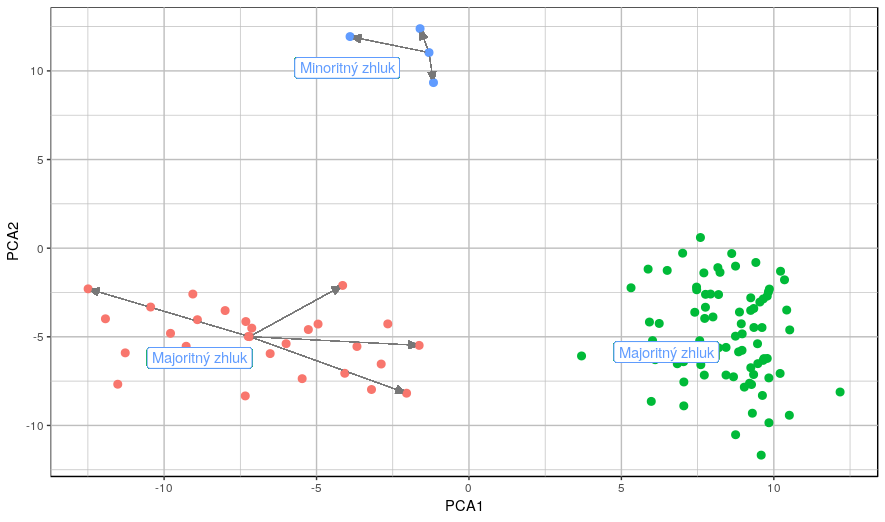
\includegraphics[width=\textwidth]{clustering_score.png}
  \caption{Skórovanie podozrivých inštancií a~zhlukov.}
  \label{fig:clustering-score}
\end{figure}

Vypočítané skóre anomálnosti je potrebné vyhodnotiť a~porovnávať navzájom voči
ostatným navrhovaným skórovaniam. V~prípade dostupnosti dát s~označenými
anomálnymi inštanciami je jednoduché pomocou vyhodnocovacích metrík
analyzovaných v~kapitole~\ref{c:evaluation-metrics} určiť presnosť daného
riešenia. Ako už bolo spomenuté, vytvorenie takéhoto datasetu je nesmierne
časovo a~finančne náročné. Vyhodnocovanie vytvoreného skóre je založené na
vhodnej reprezentácií časového radu v~dvojdimenzionálnom priestore pomocou
FeaClip reprezentácie, opísanej v~kapitole~\ref{c:feaclip-representation}
a~metódy PCA, ktorá je bližšie opísaná v~kapitole~\ref{c:dimension-reduction}.
Preto je potrebné analyzovať a~porovnať vzorku vybraných anomálnych intervalov
pri rôznych oskórovaniach navzájom a~následne zvoliť nastavenie skórovania podľa
dosiahnutých výsledkov. Na dodatočné overenie kvality skórovania môže slúžiť aj
medzikvartilové rozpätie, v~prípade, že skórovanie bude zodpovedať normálnej
distribúcií. Za anomálie budeme tak považovať intervaly, ktorých anomálne skóre
sa nachádza mimo intervalu $<Q1 - 1.5 * IQR, Q3 + 1.5 * IQR>$.

%-------------------------------------------------------------------------------
%   Chapter 4 - Experimental verification
%-------------------------------------------------------------------------------

\newpage
\section{Experimentálne overenie}
Pri experimentoch sme pracovali v~jazyku~R. Použité knižnice s~verziami sú
zobrazené pomocou tabuľky~\ref{tab:libraries}.

\begin{table}[ht]
  \centering
  \caption{Použité knižnice jazyka R.}
  \label{tab:libraries}
  \begin{tabular}{|l|l|}
    \hline
    \textbf{Názov}  &   \textbf{Použitá verzia}  \\ \hline
    AnomalyDetection    &   1.0         \\ \hline
    BreakoutDetection   &   1.0.1       \\ \hline
    cluster             &   2.0.6       \\ \hline
    clusterCrit         &   1.2.8       \\ \hline
    data.table          &   1.12.0      \\ \hline
    devtools            &   1.13.6      \\ \hline
    dplyr               &   0.7.8       \\ \hline
    dtw                 &   1.20-1      \\ \hline
    dtwclust            &   5.5.1       \\ \hline
    ggplot2             &   3.1.0       \\ \hline
    lubridate           &   1.7.4       \\ \hline
    pkgmaker            &   0.27        \\ \hline
    plotly              &   4.8.0       \\ \hline
    proxy               &   0.4-22      \\ \hline
    registry            &   0.5         \\ \hline
    rngtools            &   1.3.1       \\ \hline
    stringr             &   1.3.1       \\ \hline
    TSrepr              &   1.0.1       \\ \hline
    zoo                 &   1.8-4       \\ \hline
  \end{tabular}
\end{table}

Pri experimentoch sme použili dataset 4621 írskych domácností, ktorých spotreba
elektrickej energie bola počas 17 mesiacov sledovaná pomocou inteligentných
meračov. Dáta boli zberané každých 15 minút v~období medzi 15. júlom 2009 a~31.
decembrom 2010. Dataset obsahuje iba časovú známku, spotrebu v~kW a~príznak
sviatku. Spotreba elektrickej energie meraná v~kW nadobúda hodnoty v~intervale
$<0, 66.815>$ a~priemerná spotreba je 0.6727399 kW. Medián, dolný a~horný
kvantil je zobrazený v~tabuľke~\ref{tab:quantile}. Štandardná odchýlka súboru
je 1.372831. Je náročné prehľadne vizualizovať množstvo meraní od odberateľov,
preto sme použili čiarové a krabicové grafy~\ref{fig:whole_plot} na vizualizáciu
náhodne vybraných odberateľov.

\begin{table}[ht]
  \centering
  \caption{Charakteristiky polohy použitého datasetu.}
  \label{tab:quantile}
  \begin{tabular}{|c|c|c|}
    \hline
    \textbf{Dolný kvantil}  &   \textbf{Medián}		&		\textbf{Horný kvantil} \\ \hline
    0.121								    &   0.269							&		0.666					         \\ \hline
  \end{tabular}
\end{table}

\begin{figure}[htbp]
  \centering
  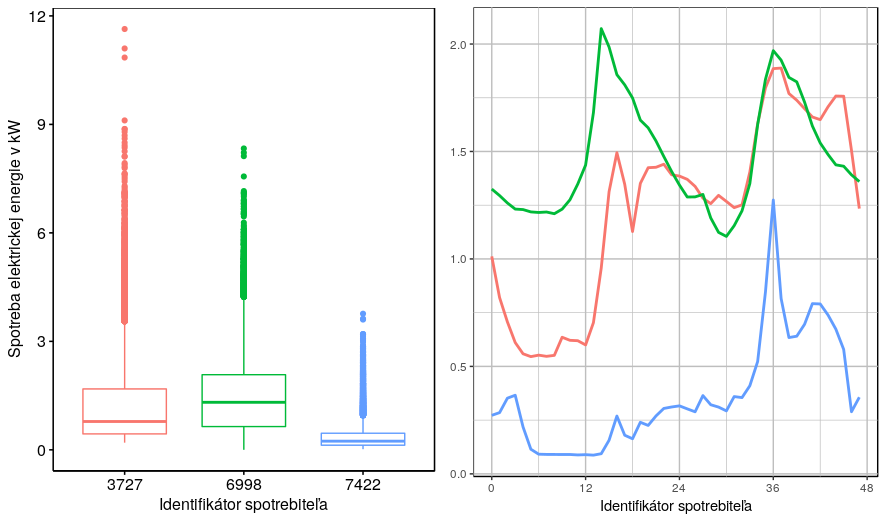
\includegraphics[width=\textwidth]{sample_plot.png}
  \caption{Krabicový graf znázorňujúci spotrebu vybraných odberateľov.}
  \label{fig:whole_plot}
\end{figure}

Profil spotrebiteľa sa výrazne líši počas pracovných dní a~víkendov, preto je
celý proces opísaný v~kapitole~\ref{c:solution-design} aplikovaný osobitne na
pracovné dni a~osobitne na dni voľna, čiže sviatky, soboty a~nedele. Cieľom je
zvýšiť presnosť zhlukovania a~následne identifikácie anomálnych intervalov
v~pôvodnom datasete. Charakteristiky polohy sú prehľadne zobrazené
v~tabuľke~\ref{tab:dataset-statistics}. Štandardná odchýlka pracovných dní je
1.418979 a~dní voľna 1.24807. Pre lepšiu vizualizáciu rozdielov medzi pracovnými
dňami a~dňami voľna sme vizualizovali spotrebu elektrickej energie rovnakých
odberateľov grafmi~\ref{fig:workdays_plot} a~\ref{fig:holidays_plot}.

\begin{table}[ht]
  \centering
  \caption{Charakteristiky polohy po rozdelení datasetu.}
  \label{tab:dataset-statistics}
  \begin{tabular}{|r|c|c|c|c|}
    \hline
					&  \textbf{Pracovné dni}  &	\textbf{Víkendy}	&	\textbf{Sviatky}	&	\textbf{Dni voľna} 	\\ \hline
		Priemer				&		0.6826072			&		0.6480718				&		0.7035064				&		0.6495951				 	\\ \hline
		Minimum				&		0							&		0								&		0								&		0								 	\\ \hline
		Dolný kvantil	&		0.121					&		0.124						&		0.127						&		0.124							\\ \hline
		Medián				&		0.266					&		0.275						&		0.303						&		0.276							\\ \hline
		Horný kvantil	&		0.644					&		0.670						&		0.778						&		0.673							\\ \hline
		Maximum				&		66.815				&		42.326					&		38.530					&		42.326						\\ \hline
  \end{tabular}
\end{table}

\begin{figure}[htbp]
  \centering
  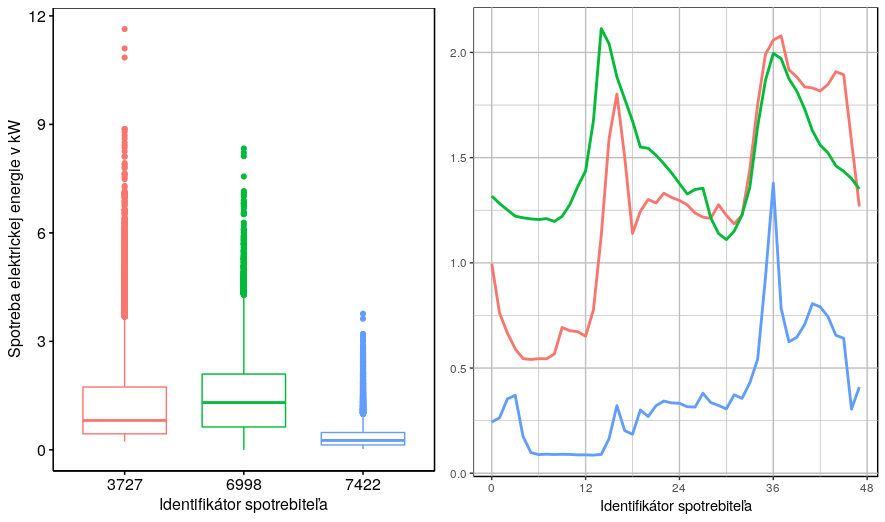
\includegraphics[width=\textwidth]{workdays_plot.png}
  \caption{Krabicový graf znázorňujúci spotrebu vybraných odberateľov počas pracovných dní.}
  \label{fig:workdays_plot}
\end{figure}

\begin{figure}[htbp]
  \centering
  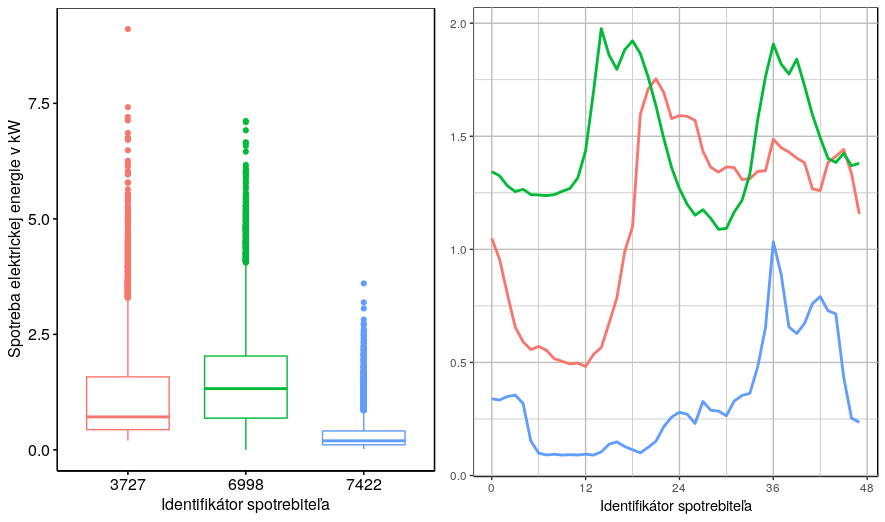
\includegraphics[width=\textwidth]{holidays_plot.png}
  \caption{Krabicový graf znázorňujúci spotrebu vybraných odberateľov počas dní voľna.}
  \label{fig:holidays_plot}
\end{figure}

\subsection{Výber hyperparametrov zhlukovania}
Zhlukovacie metódy poskytujú viacero parametrov, ktoré ovplyvňujú výsledné
zhlukovanie, jeho kvalitu alebo časovú náročnosť. Pri práci sme sa zamerali
najmä na dosahovanú presnosť, ktorú sme merali pomocou zhlukovacích validačných
indexov, bližšie opísaných v~kapitole~\ref{c:cluster-validity-indeces}. Niektoré
hyperparametre sme testovali iba na požadovanom rozmedzí. Veľkosť posuvného okna
by nemala presahovať 4-5 týždňov, aby okno neobsahovalo sezónnosť jednotlivých
ročných období. Všetky výsledky experimentov sa nachádzajú v~prílohe
v~kapitole~\ref{c:clustering-hyperparameters-experiments}. Z~vybraných
grafov~\ref{fig:cvi-sparse-sil} a~\ref{fig:cvi-dense-db} je zrejmé, že najlepším
nastavením hyperparametrov je práve nízky počet okien, ktoré budú agregované.
Výsledný počet zhlukov by mal byť približne 25. Ostatné grafy podporujú naše
tvrdenie, prípadne neposkytujú dostatočnú výpovednú hodnotu, keďže rozdiel
medzi jednotlivými pokusmi je minimálny.

\begin{figure}[htbp]
  \centering
  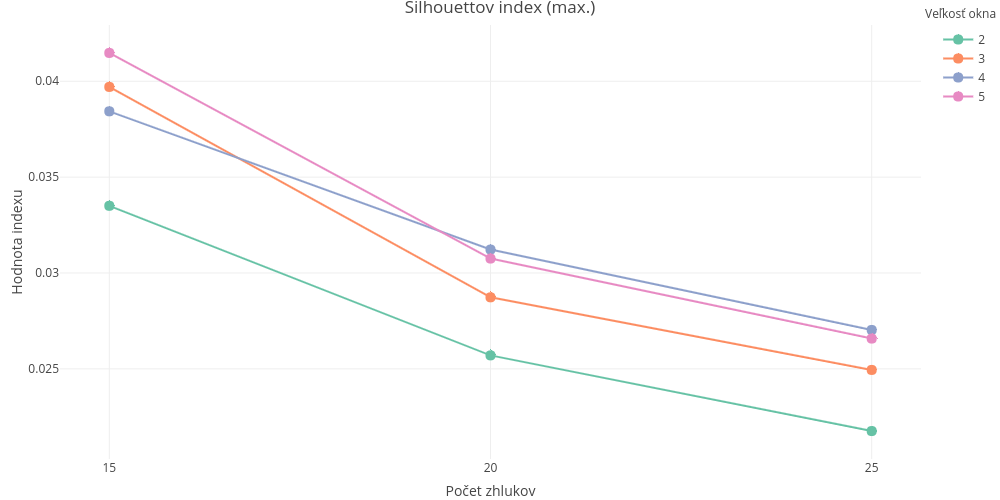
\includegraphics[width=\textwidth]{cvi/dtw_basic_workdays_sparse/201902271850-Sil-dtw_basic_workdays_sparse.png}
  \caption{Graf zhlukovania, porovnanie veľkosti posuvného okna a~počtu zhlukov.}
	\label{fig:cvi-sparse-sil}
\end{figure}
\begin{figure}[htbp]
  \centering
  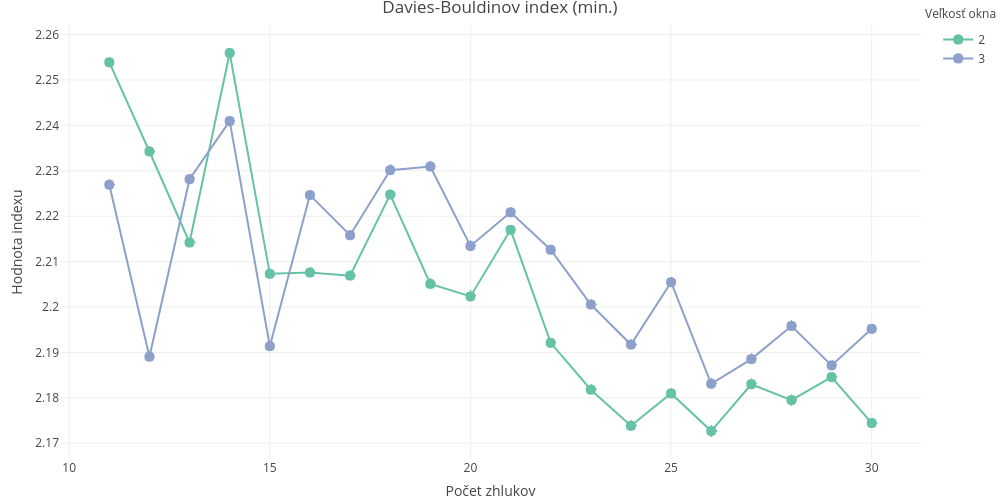
\includegraphics[width=\textwidth]{cvi/dtw_basic_workdays_dense/201902271851-DB-dtw_basic_workdays_dense.png}
  \caption{Graf zhlukovania, porovnanie veľkosti posuvného okna a~počtu zhlukov.}
	\label{fig:cvi-dense-db}
\end{figure}

Ďalším testovaným hyperparametrom sú vzdialenostné metriky, ktoré sú použité
implementované v~knižnici
\textit{dtwclust}~\footnote{https://CRAN.R-project.org/package=dtwclust}.
Metriky sú bližšie popísané v~kapitole~\ref{c:distance-metrics}.
Z~kapitoly~\ref{c:cluster-validity-indeces} je zrejmé, že najlepšiu informáciu
o~kvalite zhlukovania poskytujú práve Silhouetteov index
a~modifikovaný Davies-Bouldinov index, vizualizované na
grafoch~\ref{fig:cvi-metric-sil} a~\ref{fig:cvi-metric-dbs}. Najvhodnejšími
vzdialenostnými metrikami sú potom GAK a~DTW, pri ďalších experimentoch preto
budeme používať GAK~\ref{c:distance-metrics-gak}. Je dôležité poznamenať, že
pri rovnakom nastavení funkcie, sú výsledky medzi jednotlivými behmi nezávislé
a~rôzne. Exprimentmi sme však overili, že rozdiely sú štatisticky nevýznamné.

\begin{figure}[htbp]
  \centering
  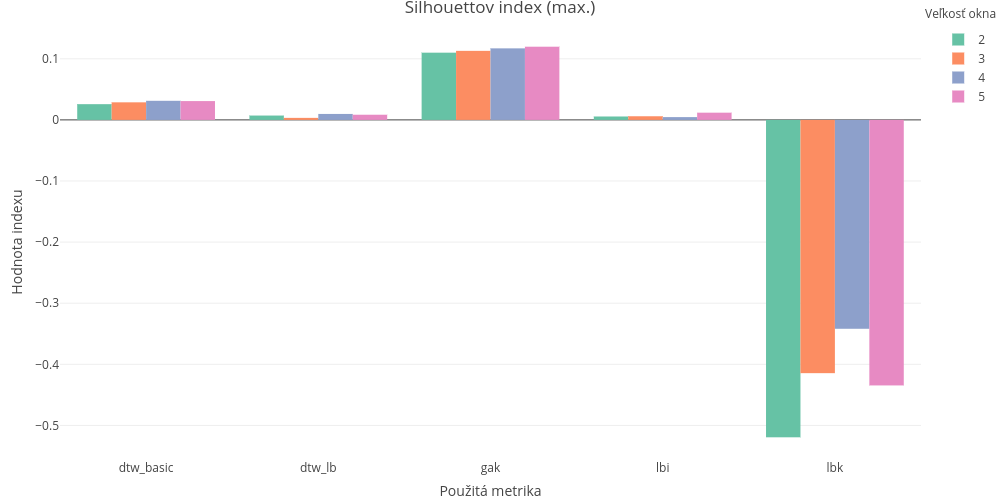
\includegraphics[width=\textwidth]{cvi/metric_comparison/201902271851-Sil-metric_comparison.png}
  \caption{Graf zhlukovania, porovnanie vzdialenostných metrík.}
	\label{fig:cvi-metric-sil}
\end{figure}
\begin{figure}[htbp]
  \centering
  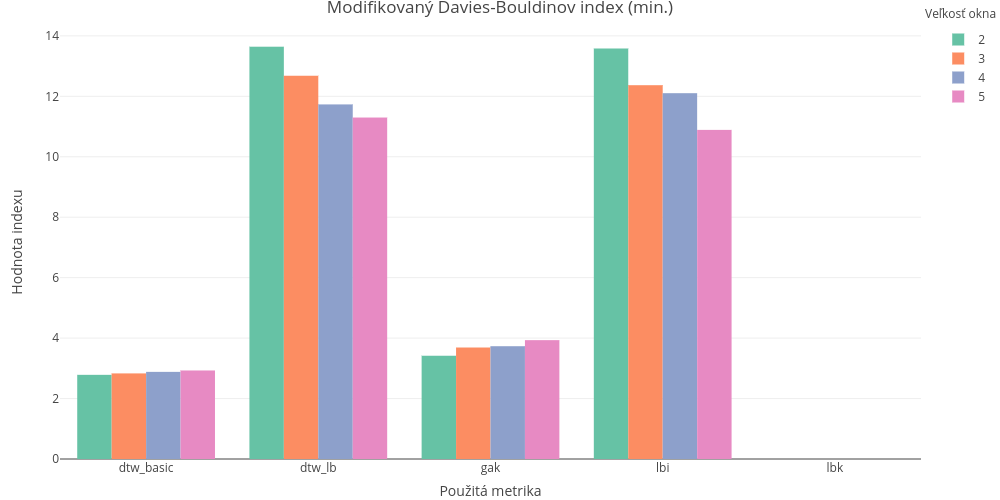
\includegraphics[width=\textwidth]{cvi/metric_comparison/201902271851-DBstar-metric_comparison.png}
  \caption{Graf zhlukovania, porovnanie vzdialenostných metrík.}
	\label{fig:cvi-metric-dbs}
\end{figure}

Dôležitým nastavením posuvného okna je jeho tvar a~posun. Pri výbere tvaru sme
sa zamerali najmä na pracovné dni, no na porovnanie sme vykonali experimenty aj
s~celými týždňami. Predpokladali sme, že zhlukovanie vytvorené iba z~pracovných
dní bude kvalitnejšie. Na grafe~\ref{fig:cvi-window-sil} si môžeme všimnúť
približne rovnaké výsledky zhlukovania s~posuvným oknom nad pracovnými dňami.
Pri veľkosti posunu sme porovnávali iba experimenty vykonané nad pracovnými
dňami. Výsledky experimentov nie sú signifikantne rozdielne, preto sme zvolili
časovo menej náročný výpočet s~posunom po týždňoch. Beh zhlukovania s~dňovým
posunom trval 5-krát dlhšie oproti týždňovému posunu.

\begin{figure}[htbp]
  \centering
  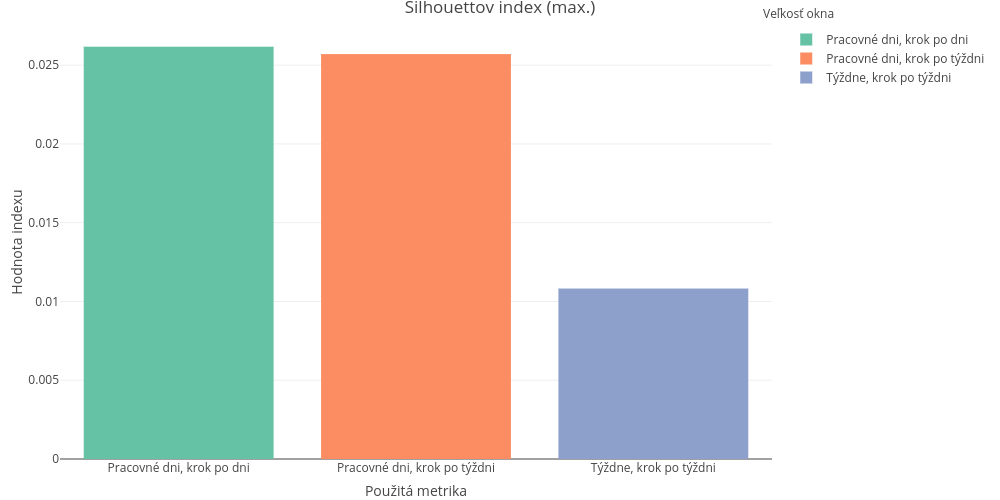
\includegraphics[width=\textwidth]{cvi/window_comparison/201903072017-Sil-window_comparison.png}
  \caption{Graf zhlukovania, porovnanie veľkostí a~typov posuvných okien.}
	\label{fig:cvi-window-sil}
\end{figure}

Predspracovanie dataset pozostáva aj z~normalizácie dát pomocou z-skóre, ktoré
je bližšie opísané v~kapitole~\ref{c:z-score}. Použitá knižnica
\textit{dtwclust}~\footnote{https://CRAN.R-project.org/package=dtwclust}
v~jazyku R~poskytuje taktiež predspracovanie vstupnej množiny dát pomocou
rovnakej normalizácie. Preto sme vykonali niekoľko experimentov pre porovnanie
časovej náročnosti a~presnosti výsledného zhlukovania, pri použití vstavanej
a~externej normalizácie. Časová náročnosť pri použití oboch normalizácií súčasne
alebo iba jednej z~nich bola približne rovnaká. Rozdiel bol vo výsledkoch, ktoré
nepoužívali externú normalizáciu. V~prípade použitia oboch súčasne alebo iba
externej normalizácie sú dosahované výsledky porovnateľné.

%-------------------------------------------------------------------------------
%   Chapter 8 - Bibliography
%-------------------------------------------------------------------------------

\newpage
\bibliographystyle{iso-690/slovakiso}
\bibliography{bibliography}
\newpage\null\thispagestyle{empty}\newpage

%-------------------------------------------------------------------------------
%   Appendix
%-------------------------------------------------------------------------------

\begin{appendices}
\newpage
\section{Obsah elektronického média}
\dirtree{%
  .1 CD nosič.
  .2 \textbf{doc}.
	.3 DP\_MATUS\_CUPER.pdf.
  .2 \textbf{src}.
  .3 aggregators.R.
  .3 analyzators.R.
  .3 anomalyDetectors.R.
  .3 boilerplate.R.
  .3 filters.R.
  .3 loaders.R.
  .3 oneliners.sh.
  .3 presentation.R.
  .3 ts-sample-decomposition.R.
  .3 utilities.R.
  .3 visualizators.R.
}

\begin{description}
  \item[$\bullet$ doc] dokumentácia, obrázky použité v nej a zdrojové súbory pre LaTeX
  \item[$\bullet$ src] skripty, prototypy a časti zdrojových kódov, ktoré boli použité pri experimentoch
\end{description}


\newpage
\section{Vizualizácie experimentov pre výber hyperparametrov}
\label{c:clustering-hyperparameters-experiments}
Každý index obsahuje aj informáciu o~jeho optimálnych hodnotách. Pri indexoch,
ktoré obsahujú $(max.)$ znamenajú väčšie hodnoty lepšie výsledné zhlukovanie.
Pri indexoch s~$(min.)$ nižšie hodnoty znamenajú lepšie výsledky zhlukovania.

\begin{figure}[htbp]
  \centering
  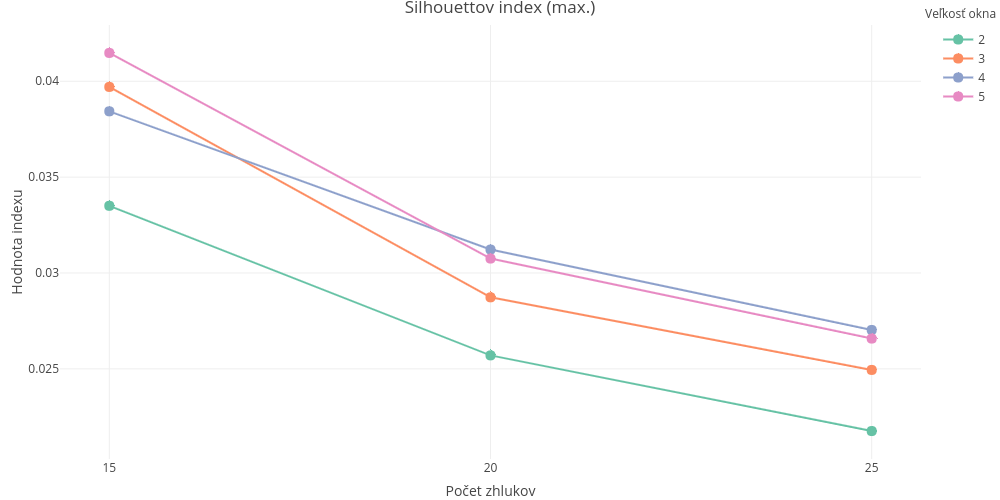
\includegraphics[width=\textwidth]{cvi/dtw_basic_workdays_sparse/201902271850-Sil-dtw_basic_workdays_sparse.png}
  \caption{Graf zhlukovania, porovnanie veľkosti posuvného okna a~počtu zhlukov.}
\end{figure}
\begin{figure}[htbp]
  \centering
  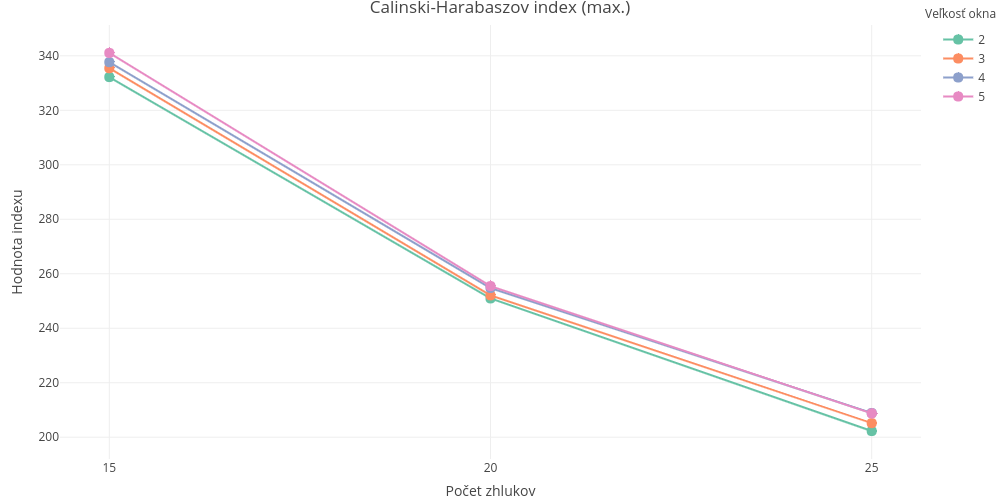
\includegraphics[width=\textwidth]{cvi/dtw_basic_workdays_sparse/201902271850-CH-dtw_basic_workdays_sparse.png}
  \caption{Graf zhlukovania, porovnanie veľkosti posuvného okna a~počtu zhlukov.}
\end{figure}
\begin{figure}[htbp]
  \centering
  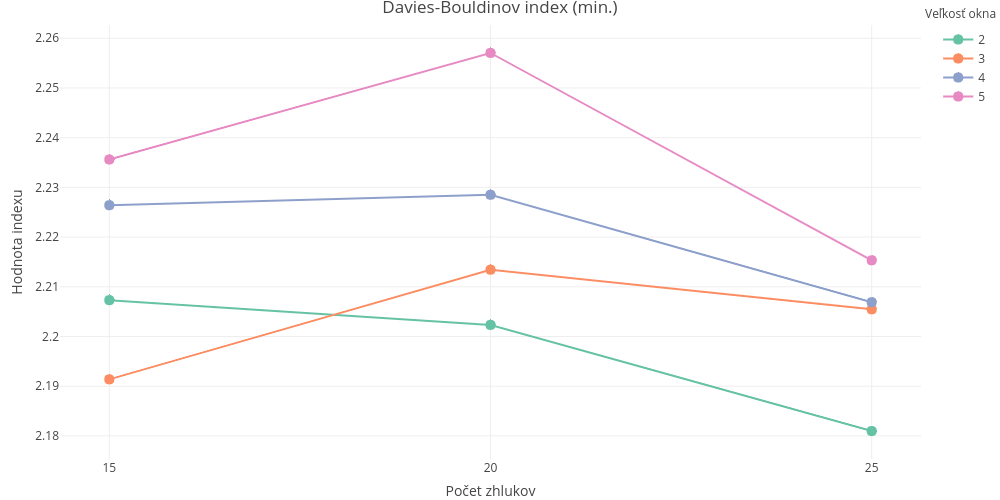
\includegraphics[width=\textwidth]{cvi/dtw_basic_workdays_sparse/201902271850-DB-dtw_basic_workdays_sparse.png}
  \caption{Graf zhlukovania, porovnanie veľkosti posuvného okna a~počtu zhlukov.}
\end{figure}
\begin{figure}[htbp]
  \centering
  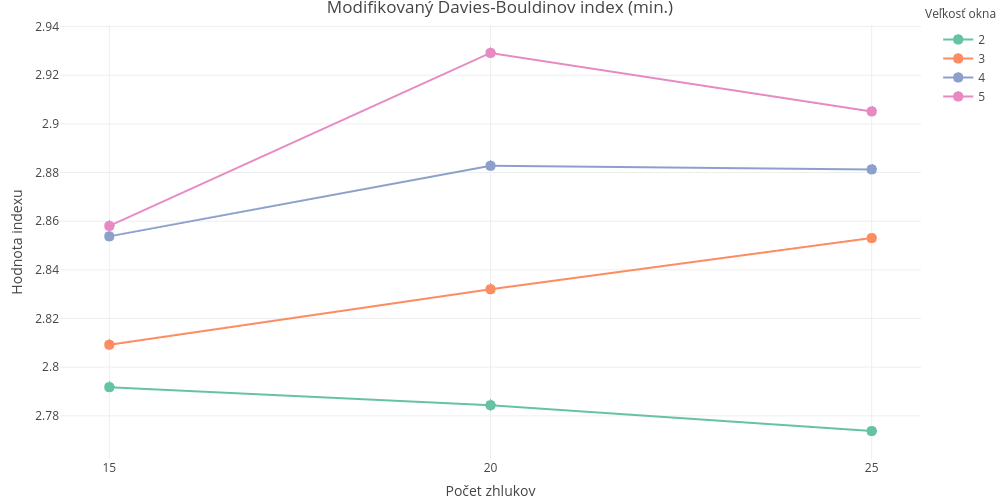
\includegraphics[width=\textwidth]{cvi/dtw_basic_workdays_sparse/201902271850-DBstar-dtw_basic_workdays_sparse.png}
  \caption{Graf zhlukovania, porovnanie veľkosti posuvného okna a~počtu zhlukov.}
\end{figure}

\begin{figure}[htbp]
  \centering
  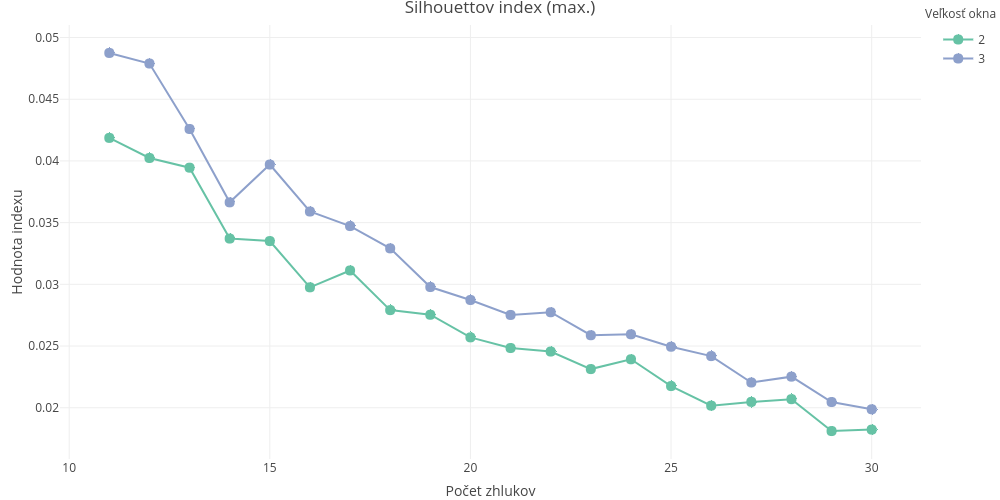
\includegraphics[width=\textwidth]{cvi/dtw_basic_workdays_dense/201902271851-Sil-dtw_basic_workdays_dense.png}
  \caption{Graf zhlukovania, porovnanie veľkosti posuvného okna a~počtu zhlukov.}
\end{figure}
\begin{figure}[htbp]
  \centering
  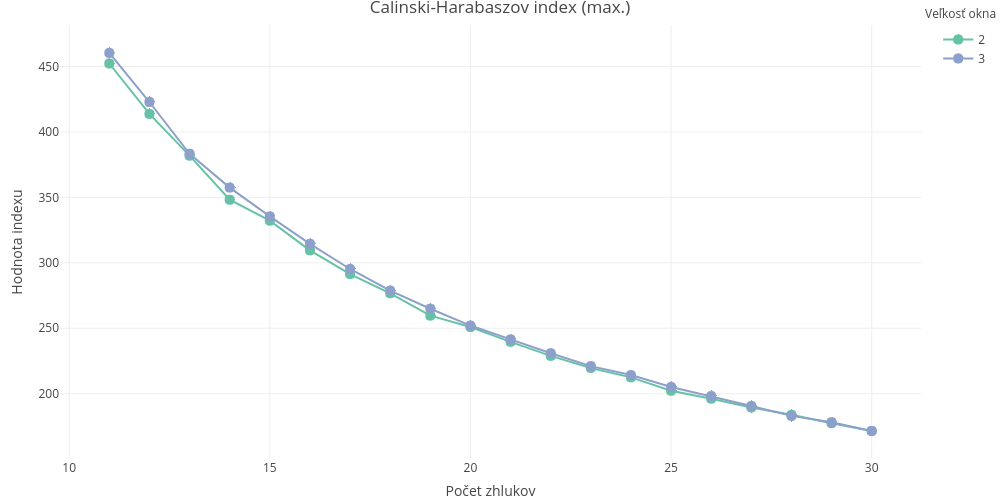
\includegraphics[width=\textwidth]{cvi/dtw_basic_workdays_dense/201902271851-CH-dtw_basic_workdays_dense.png}
  \caption{Graf zhlukovania, porovnanie veľkosti posuvného okna a~počtu zhlukov.}
\end{figure}
\begin{figure}[htbp]
  \centering
  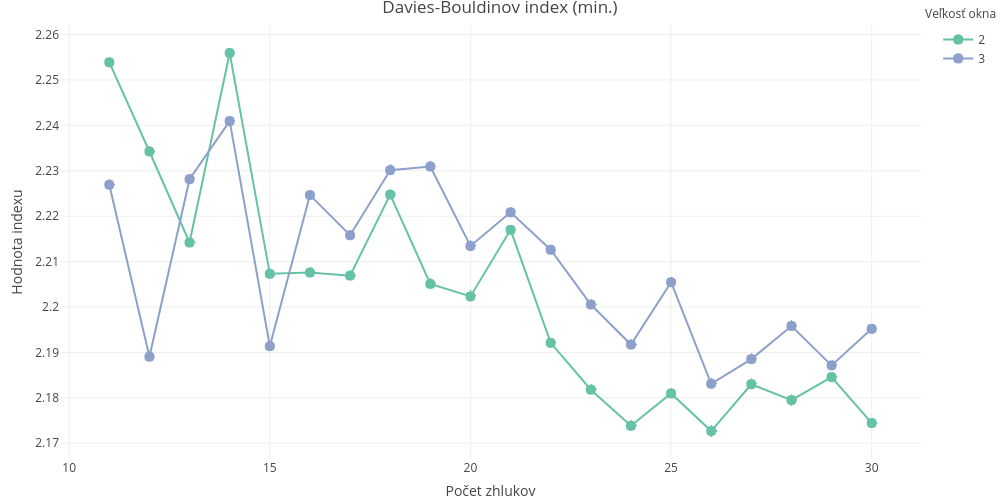
\includegraphics[width=\textwidth]{cvi/dtw_basic_workdays_dense/201902271851-DB-dtw_basic_workdays_dense.png}
  \caption{Graf zhlukovania, porovnanie veľkosti posuvného okna a~počtu zhlukov.}
\end{figure}
\begin{figure}[htbp]
  \centering
  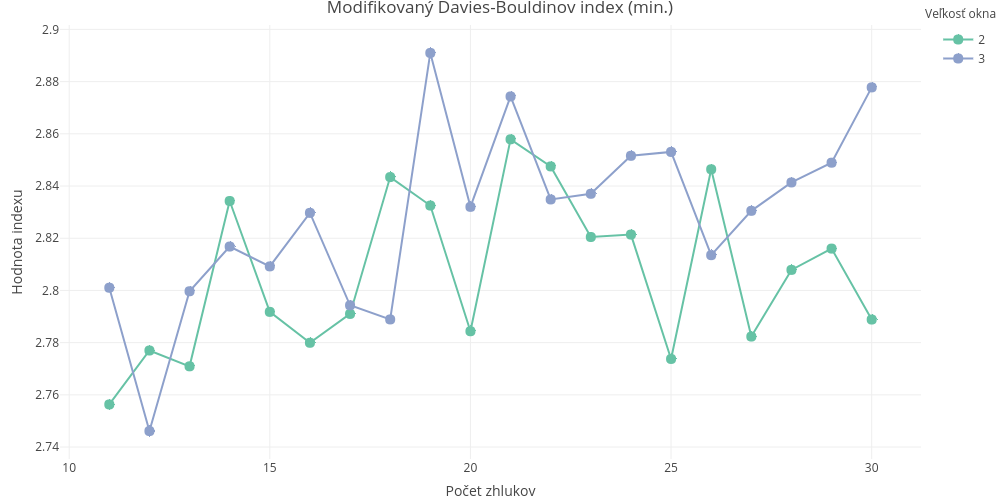
\includegraphics[width=\textwidth]{cvi/dtw_basic_workdays_dense/201902271851-DBstar-dtw_basic_workdays_dense.png}
  \caption{Graf zhlukovania, porovnanie veľkosti posuvného okna a~počtu zhlukov.}
\end{figure}

\begin{figure}[htbp]
  \centering
  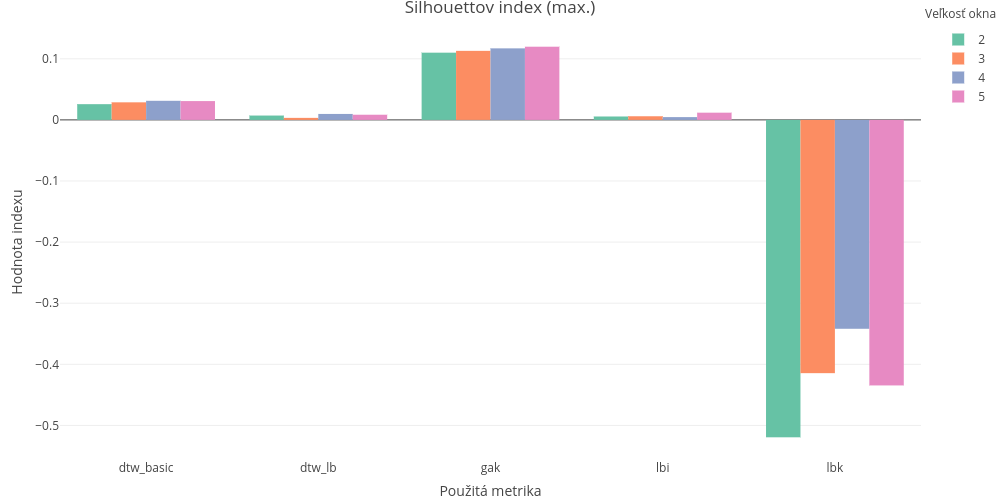
\includegraphics[width=\textwidth]{cvi/metric_comparison/201902271851-Sil-metric_comparison.png}
  \caption{Graf zhlukovania, porovnanie vzdialenostných metrík.}
\end{figure}
\begin{figure}[htbp]
  \centering
  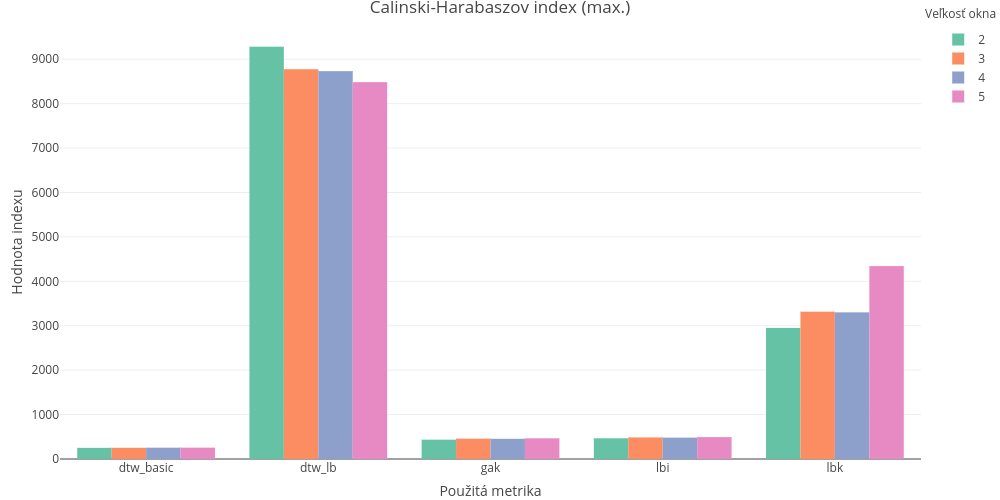
\includegraphics[width=\textwidth]{cvi/metric_comparison/201902271851-CH-metric_comparison.png}
  \caption{Graf zhlukovania, porovnanie vzdialenostných metrík.}
\end{figure}
\begin{figure}[htbp]
  \centering
  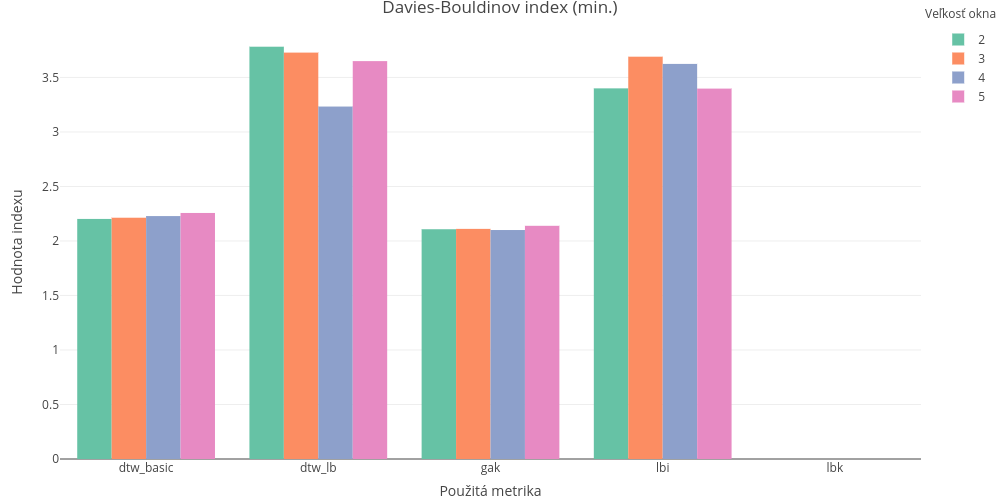
\includegraphics[width=\textwidth]{cvi/metric_comparison/201902271851-DB-metric_comparison.png}
  \caption{Graf zhlukovania, porovnanie vzdialenostných metrík.}
\end{figure}
\begin{figure}[htbp]
  \centering
  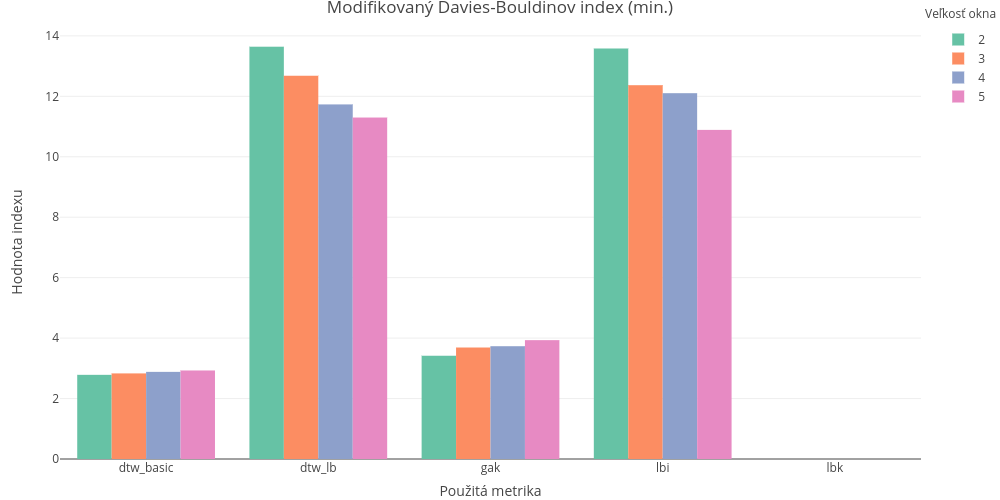
\includegraphics[width=\textwidth]{cvi/metric_comparison/201902271851-DBstar-metric_comparison.png}
  \caption{Graf zhlukovania, porovnanie vzdialenostných metrík.}
\end{figure}

\begin{figure}[htbp]
  \centering
  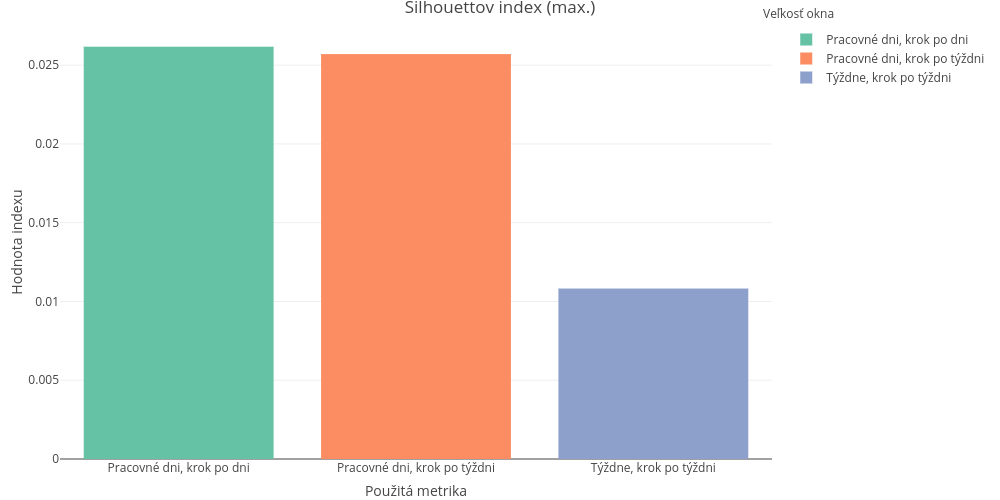
\includegraphics[width=\textwidth]{cvi/window_comparison/201903072017-Sil-window_comparison.png}
  \caption{Graf zhlukovania, porovnanie veľkostí a~typov posuvných okien.}
\end{figure}
\begin{figure}[htbp]
  \centering
  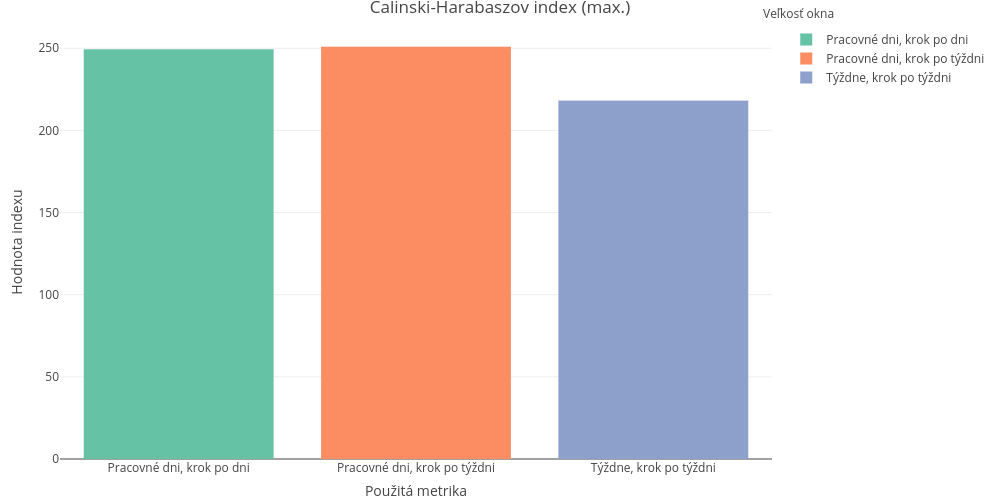
\includegraphics[width=\textwidth]{cvi/window_comparison/201903072017-CH-window_comparison.png}
  \caption{Graf zhlukovania, porovnanie veľkostí a~typov posuvných okien.}
\end{figure}
\begin{figure}[htbp]
  \centering
  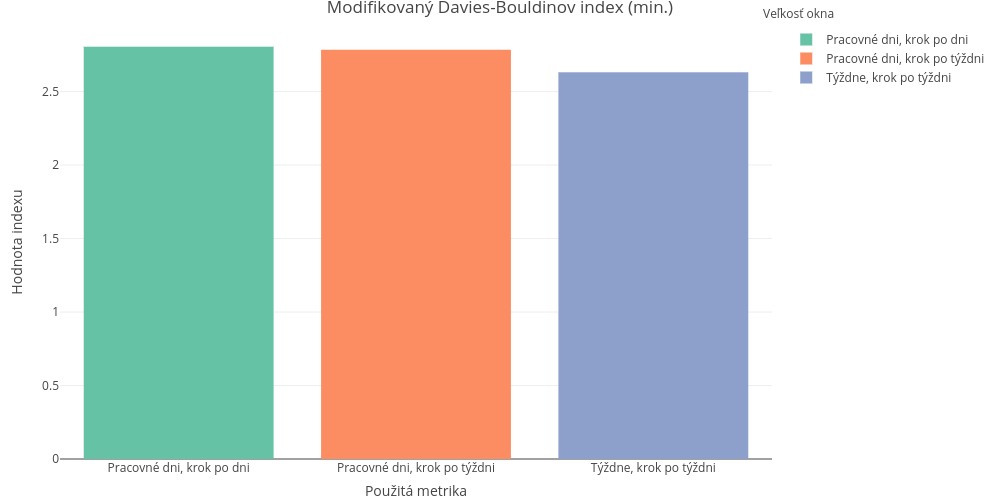
\includegraphics[width=\textwidth]{cvi/window_comparison/201903072017-DBstar-window_comparison.png}
  \caption{Graf zhlukovania, porovnanie veľkostí a~typov posuvných okien.}
\end{figure}
\begin{figure}[htbp]
  \centering
  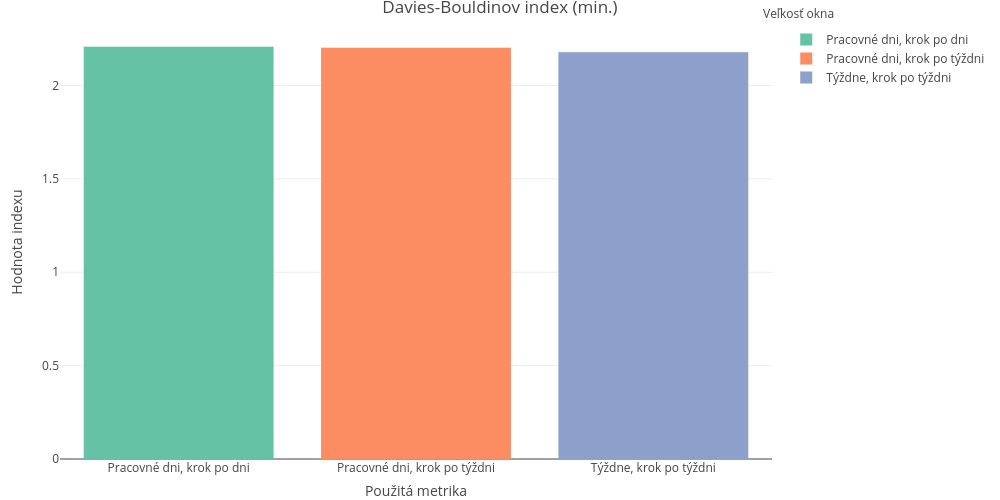
\includegraphics[width=\textwidth]{cvi/window_comparison/201903072017-DB-window_comparison.png}
  \caption{Graf zhlukovania, porovnanie veľkostí a~typov posuvných okien.}
\end{figure}


\end{appendices}

\end{document}
